\documentclass[journal]{IEEEtran}
\IEEEoverridecommandlockouts

\usepackage{cite}
\usepackage{amsmath,amssymb,amsfonts}
\usepackage{algorithmic}
\usepackage{graphicx}
\usepackage{textcomp}
\usepackage{xcolor}
\usepackage[english,spanish]{babel}
\usepackage{blindtext}
\usepackage{comment}

\graphicspath{ {images/} }
\def\BibTeX{{\rm B\kern-.05em{\sc i\kern-.025em b}\kern-.08em
    T\kern-.1667em\lower.7ex\hbox{E}\kern-.125emX}}

% thebibliography fix
\makeatletter
\def\endthebibliography{%
	\def\@noitemerr{\@latex@warning{Empty `thebibliography' environment}}%
	\endlist
}
\makeatother

\begin{document}
\selectlanguage{spanish}

% Comentarios
% - Las frases de sentido común están prohibidas
% - Una frase no referenciada significa que es un resultado de la investigación del autor.
% - Un argumento ya existente necesita solamente un resumen si es útil para la investigación. Ej: sección "tema específico".
% Todo referenciado con artículos o libros.
% - Cada frase, si no es el resultado de una investigación, necesita una referencia.
% - Si al finalizar el paper una sección no se utilizó, se puede quitar esa sección.
% - El paper se escribe en tiempo presente.
% - Si no es un resultado de la investigación, entonces es un dato y necesita una referencia.
% - Las secciones se pueden leer independientemente, sin saber las secciones anteriores o las siguientes. No referenciar secciones.
%- Evitar introducir un argumento o un concepto a nivel histórico. Poner directamente las fórmulas o el hecho necesario a la investigación.

\title{
    Propuesta de solución de LMS orientado al microaprendizaje para su uso en organizaciones\\
    %{\footnotesize \textsuperscript{*}...}
    %\thanks{...}
}

\author{
    \IEEEauthorblockN{Andrés Isaac Biso}
    \IEEEauthorblockA{
        \textit{Facultad de Ingeniería} \\
        \textit{Universidad de Palermo}\\
        Ciudad Autónoma de Buenos Aires, Argentina \\
    }
}
\maketitle

% Sección obligatoria.
% ¿Cómo debe escribirse esta sección?
% Está formado por dos párrafos, uno para la motivación/problemática y otro para
% la idea, donde se contextualiza la investigación del paper. La idea debe estar
% escrita desde un punto de vista técnico. Debe contener la conclusión de la
% investigación (forma resumida).
\begin{abstract}
    En la actualidad, la falta de tiempo disponible representa un desafío para
    la educación. En el entorno laboral, las personas deben equilibrar múltiples
    responsabilidades, lo que limita su capacidad para participar en procesos de
    formación extensos. A medida que la tecnología, la economía y la sociedad
    evolucionan rápidamente, surge la necesidad de enfoques educativos
    alternativos, que permitan adquirir conocimientos en períodos cortos sin
    comprometer su calidad. En este contexto, el microaprendizaje ofrece una
    solución flexible y accesible, facilitando el acceso a información concisa y
    adaptada a las necesidades individuales de cada empleado.

    Este trabajo presenta el desarrollo de una solución web de capacitación
    empresarial basada en microaprendizaje, diseñada para optimizar el tiempo de
    los empleados sin afectar la continuidad de su formación. La solución adapta
    los contenidos según el tiempo disponible y los objetivos de cada usuario,
    promoviendo un desarrollo profesional constante. A través de actividades
    breves, como videos, lecturas y cuestionarios interactivos, se garantiza un
    aprendizaje eficiente y accesible desde cualquier dispositivo.
    
    Los resultados obtenidos demuestran que la implementación de esta solución
    ha mejorado significativamente la retención del conocimiento y la aplicación
    de habilidades en el entorno laboral. La personalización del contenido y la
    accesibilidad multiplataforma han favorecido la continuidad en la formación,
    permitiendo que los empleados progresen en sus rutas de aprendizaje sin
    interrupciones. Además, se ha observado un impacto positivo en la eficiencia
    del aprendizaje y el crecimiento profesional, evidenciando que el
    microaprendizaje es una estrategia efectiva para la capacitación
    empresarial.
\end{abstract}

\begin{IEEEkeywords}
	informal learning, microlearning, microcontent, online communities, Web 2.0,
	e-learning
\end{IEEEkeywords}

\section{Introduccíon}
% Sección obligatoria.
% ¿Qué escribir en esta sección?
% Motivación (o problemática), se incluyen los antecedentes y una descripción técnica y detallada de la idea.
% Por último, se debe incluir una descripción del resto de las secciones del paper.
% Esta sección y marco teórico deben contener casi todas las referencias del paper.

% La problemática o motivación del paper es el inicio de la introducción y sirve para saber si el problema que plantea el paper es conocido,
% investigado y cuál es su impacto en el mundo real.
% En esa parte de la introducción es necesario incluir referencias para identificar la problemática.

% Luego de plantear la problemática, es necesario encuadrar las soluciones ya existentes para el problema así como la nueva tecnología que podría ayudar a
% solucionar el tema.
% En la introducción no se explica cómo funcionan los algoritmos, solamente se citan para entender la complejidad.

% La idea debe comenzar con: “En este trabajo, vamos a desarrollar…”, “El objetivo del paper es…”, “En este artículo se explican…"
% Escribir ¿De qué se trata su trabajo?

% La descripción de las secciones debe ser un parrafo con una descripción breve de las secciones.

% ¿Cómo debe escribirse esta sección?
% Abarca mínimo media página (idealmente debería finalizar casi al final de la página 1).

% \IEEEPARstart{E}{ste} paper desarrolla la siguiente idea.

\subsection{Problemática}
% Esta sección es conocida como "Motivación" o "Problemática".

En el mundo actual, las personas se enfrentan a una escasez de tiempo más que
nunca. La aparición de diversas preocupaciones ha limitado la posibilidad de un
enfoque a largo plazo. En esta situación, la mejor manera de mejorar el sistema
educativo es utilizar un método que proporcione la mayor cantidad de información
en el menor tiempo posible.
\cite{article:microlearning_today_students_nikkhoo}

Los cambios tecnológicos, económicos y sociales actuales impulsan la necesidad
de nuevos conceptos y estrategias para apoyar el aprendizaje permanente. La
educación, incluida la formación en el trabajo, necesita transformaciones que
requieren renovación y formas innovadoras de adaptarse adecuadamente a nuestra
forma de vivir, trabajar y aprender hoy.
\cite{article:microlearning_buchem}

Los términos que describen cómo trabajamos y aprendemos hoy, como ''trabajadores
del conocimiento'' (''knowledge workers''), ''nativos digitales'' (''Digital
Natives''), ''inmigrantes digitales'' ("Digital Immigrants"), ''estudiantes del
nuevo milenio'' (''new millennium learners'') y la ''Generación Net'' (''Net
Generation''), reflejan algunos cambios esenciales en las sociedades modernas,
''donde las tecnologías digitales forman parte inseparable de la vida cotidiana''
(''where digital technologies form an inextricable part of daily life''). El
estilo de vida de la nueva generación, es decir, de los nacidos a partir de la
década de 1980, pero también de las generaciones anteriores, se está viendo
fuertemente influenciado por Internet y las tecnologías relacionadas. Tanto los
estudiantes jóvenes como los mayores llevan sus portátiles a clases o reuniones
de trabajo, usan teléfonos móviles e internet para fomentar las redes sociales,
emplean dispositivos digitales para jugar y crear contenido, o realizan
múltiples tareas simultáneamente.
\cite{article:microlearning_buchem}

Estas nuevas tecnologías digitales que permiten la creación de contenido
generado por el usuario han dado lugar a una tendencia hacia los microformatos
(''microformats''), es decir, información breve, sencilla y específica. Junto con
los sistemas de publicación personal, como blogs o wikis, se ha vuelto bastante
fácil para cualquiera crear su propio contenido, incluido el microcontenido
(''microcontent''). El microcontenido, es decir, ''información publicada en formato
breve'', se relaciona más con un "enfoque formal de cómo presentar" el contenido
que con la calidad inherente del contenido en sí. Algunos ejemplos de
microcontenido son los podcasts, las entradas de blog, las páginas wiki o los
mensajes cortos en Facebook o X. La creación, publicación y compartición de
microcontenido en la web abre nuevas posibilidades para formas de aprendizaje
implícitas, informales e incidentales, como el microaprendizaje
(''microlearning''), término que se refiere a actividades breves de aprendizaje
con microcontenido.
\cite{article:microlearning_buchem}

\subsection{Antecedentes}
% Esta sección es conocida como "Antecedentes" o "Estado del Arte".

% Por ejemplo, si se habla de los algoritmos de ruteo, en esa sección se
% detallarán cuáles son los últimos algoritmos implementados para la comunidad
% científica. En esta sección, se explica solamente lo que ya existe y se hace
% un resumen: entonces se incluyen muchas referencias y ninguna frase o párrafo
% sobre la idea que se va a proponer.

El aprendizaje electrónico (''e-learning'') se ha convertido en una fuerza importante en el
mercado de la educación superior, con un valor de 325 mil millones de dólares
para el 2025 (Shah, 2023). El microaprendizaje consiste en enseñar contenido breve
pero lógicamente completo (Jomah et al., 2016). Según el informe de Clark et al.
(2023), la creciente tendencia del microaprendizaje surgió para cubrir la brecha
entre la creciente demanda de mano de obra cualificada por parte de las
industrias y la continua incapacidad de la educación superior para ofrecer
exalumnos "listos para el rendimiento". La pandemia de COVID-19 contribuyó a
esta tendencia desde una perspectiva diferente. Los estudiantes tenían
dificultades para comprender material complejo en casa sin interacciones
frecuentes de preguntas y respuestas (Wiley University Services, 2023). Dividir
el material en partes más pequeñas y fáciles de comprender con retroalimentación
rápida (pruebas) ayudó a los estudiantes a mantenerse atentos y motivados
durante largos períodos de distanciamiento social (Søzmen et al., 2023).

Leong et al. (2021) revisaron la literatura sobre microaprendizaje entre 2006 y
2019. Los autores identificaron 476 publicaciones relevantes sobre el tema.
Comenzó como una metodología de transferencia de conocimientos basada en el
trabajo, el aprendizaje. En la última década, el concepto de microaprendizaje se
ha vuelto ampliamente conocido y famoso. El informe del Sistema Universitario
Global de Canadá (2022) señaló las deficiencias de la educación presencial
tradicional y cómo la educación flexible y basada en habilidades puede
abordarlas. En busca de relevancia, las instituciones encontraron que el
microaprendizaje era relevante para su adopción en la educación superior (Leong
et al., 2021).

Shatte y Teague (2020) investigaron la literatura sobre microaprendizaje basado
en tecnología en la educación superior. Los autores muestran la contribución del
enfoque de microaprendizaje al aumento de los resultados educativos. Los
estudiantes reportaron una mayor motivación y un mayor compromiso con el
material y los procesos de aprendizaje al estudiar porciones pequeñas y concisas
de material (Shatte y Teague). Garshasbi et al. (2021) analizaron el efecto del
microaprendizaje en la enseñanza de las disciplinas STEM (ciencia, tecnología,
ingeniería y matemáticas). En un mundo con abundante información, la capacidad
de los estudiantes para concentrarse en clases virtuales, ya sea en línea o
presenciales, es cuestionable. El microaprendizaje podría ser una solución
adecuada para abordar este desafío. En la educación en línea, una pequeña
porción de material, con un enfoque lógico y concluyente, preparada para su
entrega o consumo por parte de los estudiantes ha demostrado ser una forma
eficaz de transferencia de conocimiento (Garshasbi et al.).
\cite{article:elearning_future_trends_shahid}

\subsection{Idea}
En este trabajo, vamos a desarrollar una solución web de capacitación empresarial que incorpora el microaprendizaje
personalizado para optimizar el tiempo que los empleados dedican al mismo.
La misma, busca una experiencia de capacitación flexible y personalizada, adaptándose al tiempo disponible de cada empleado.
Además, las rutas de aprendizaje se ajustan a los objetivos individuales, fomentando el desarrollo profesional de manera constante.
El objetivo del paper es analizar cómo esta plataforma, mediante actividades breves como videos, lecturas y cuestionarios,
logra un aprendizaje eficiente adaptado a las necesidades individuales de los empleados.
En este artículo, se explican los beneficios de la accesibilidad multiplataforma, que garantiza continuidad en el proceso formativo,
y los efectos positivos que este enfoque ha demostrado tener en la eficiencia del aprendizaje y el crecimiento profesional.

\subsection{Secciones}

En \textbf{Introducción}, se plantea la problemática, se contextualiza con antecedentes y se presenta la idea central del trabajo.
En \textbf{Objetivos} se define las metas de la investigación, centrándose en mejorar la eficiencia del aprendizaje corporativo.
En \textbf{Justificación}, se argumenta la relevancia del enfoque, respaldado por estudios previos.
En \textbf{Marco Teórico} se profundizan los conceptos clave y marca diferencias con otros enfoques educativos.
En \textbf{Trabajos Relacionados} se revisan herramientas similares y metodologías aplicadas en otros entornos empresariales.
En \textbf{Enfoque Propuesto} se describe la solución a ser desarrollada y la arquitectura de software a ser utilizada.
En \textbf{Diseño de la Investigación} se detalla la metodología utilizada para evaluar la efectividad del sistema.
En \textbf{Instrumentos} se presentan las herramientas utilizadas, como frameworks tecnológicos y plataformas de desarrollo.
En \textbf{Componentes} se listan los elementos clave del sistema a nivel software. Se vuelve a mencionar la arquitectura pero desde la implementación.
En \textbf{Procedimientos} se explica los pasos para la implementación de la solución.
En \textbf{Resultados} se analiza el impacto del sistema, describiendo métricas y pruebas realizadas.
En \textbf{Conclusión}, se evalúan los hallazgos obtenidos y se destacan las contribuciones del modelo de microaprendizaje personalizado.
En \textbf{Apéndices} se recopila información complementaria relevante.
En \textbf{Reconocimientos}, se agradecen contribuciones significativas al proyecto.
En \textbf{Referencias} se documentan fuentes y estudios clave que sustentan la investigación.
En \textbf{Biografía}, se presenta el perfil del autor.


\section{Objetivos}
\blindtext

\section{Justificación}
\blindtext

\section{Marco Teórico}
\blindtext

\section{Trabajos Relacionados}
\blindtext
% Los trabajos relacionados podrían ser herramientas que ya existen
% o que se mencionan en los paper que hacen parte de lo mencionado en el paper.

\section{Enfoque Propuesto}
\blindtext

\section{Diseño de la investigación}
\blindtext

\section{Instrumentos}
% La sección de Instrumentos contiene: github, editor de texto, herramientas
% utilizadas, frameworks,…
\subsection{Implementación y Herramientas Tecnológicas}

El desarrollo de  la \textit{''propuesta de solución de LMS orientado al
microaprendizaje para su uso en organizaciones''} se llevó a cabo bajo un entorno
estructurado que garantizó una implementación modular y escalable. A
continuación, se detallan las principales herramientas empleadas.

\subsection{Entorno de Desarrollo}
El sistema fue desarrollado en \textbf{macOS Sequoia 15 (x64, Intel)},
utilizando \textit{Homebrew} como gestor de paquetes. Este entorno proporcionó
estabilidad y compatibilidad con las tecnologías seleccionadas.

\subsection{Lenguajes y Frameworks}
Para la implementación de los diferentes módulos del sistema, se utilizaron las
siguientes tecnologías:
\begin{itemize}
	\item \textbf{Node.js} con \textit{Express.js}: Desarrollo del servidor
	backend.
	\item \textbf{Python} con \textit{Flask}: Implementación de la lógica del
	bot y su servidor.
	\item \textbf{React.js}: Desarrollo de la interfaz de usuario del cliente.
\end{itemize}

\subsection{Contenedores y Orquestación}
Con el objetivo de garantizar la modularidad y despliegue eficiente de los
servicios, se utilizó \textbf{Docker} en conjunto con \textbf{Docker Compose}.
Esto permitió la ejecución de componentes en entornos aislados y replicables.

\subsection{Servicios Adicionales}
Se integraron diversas herramientas para la gestión de datos y almacenamiento:
\begin{itemize}
	\item \textbf{MongoDB \& Mongo Express}: Base de datos NoSQL y herramienta
	de administración.
	\item \textbf{MinIO (API \& WebUI)}: Almacenamiento distribuido de objetos.
	\item \textbf{Mailpit (SMTP \& WebUI)}: Servidor de pruebas de correo
	electrónico.
	\item \textbf{DiceBear}: Generador de avatares dinámicos.
\end{itemize}

\subsection{Implementación y Despliegue}
La ejecución del sistema sigue un flujo estructurado que involucra la
instalación de dependencias, la configuración de contenedores y la puesta en
marcha de servicios. 

Para la gestión de la base de datos, se empleó \textbf{MongoDB Compass} y
\textbf{MongoDB Express}.

\subsection{Repositorio del Proyecto}
El código fuente y la documentación del proyecto están alojados en Github. Se
pueden encontrar en el siguiente repositorio:

\begin{center}
	\textbf{\href{https://github.com/andresbiso/2025\_1C\_TFG}{https://github.com/andresbiso/2025\_1C\_TFG}}
\end{center}


\section{Componentes}
% Cuando se desarrolla una idea de un prototipo, se necesita una sección donde listar los distintos componentes hardware o software que se utilizará en el proceso de investigación.
% En los componentes hardware normalmente se encuentran los sensores. Los componentes software están más orientados a la arquitectura y
% al diseño de las aplicaciones, y no a los framework y lenguaje utilizados.

\section{Procedimientos}
\blindtext

\begin{figure*}[htbp] % Spans both columns, making it useful for large images or diagrams.
    \centering
    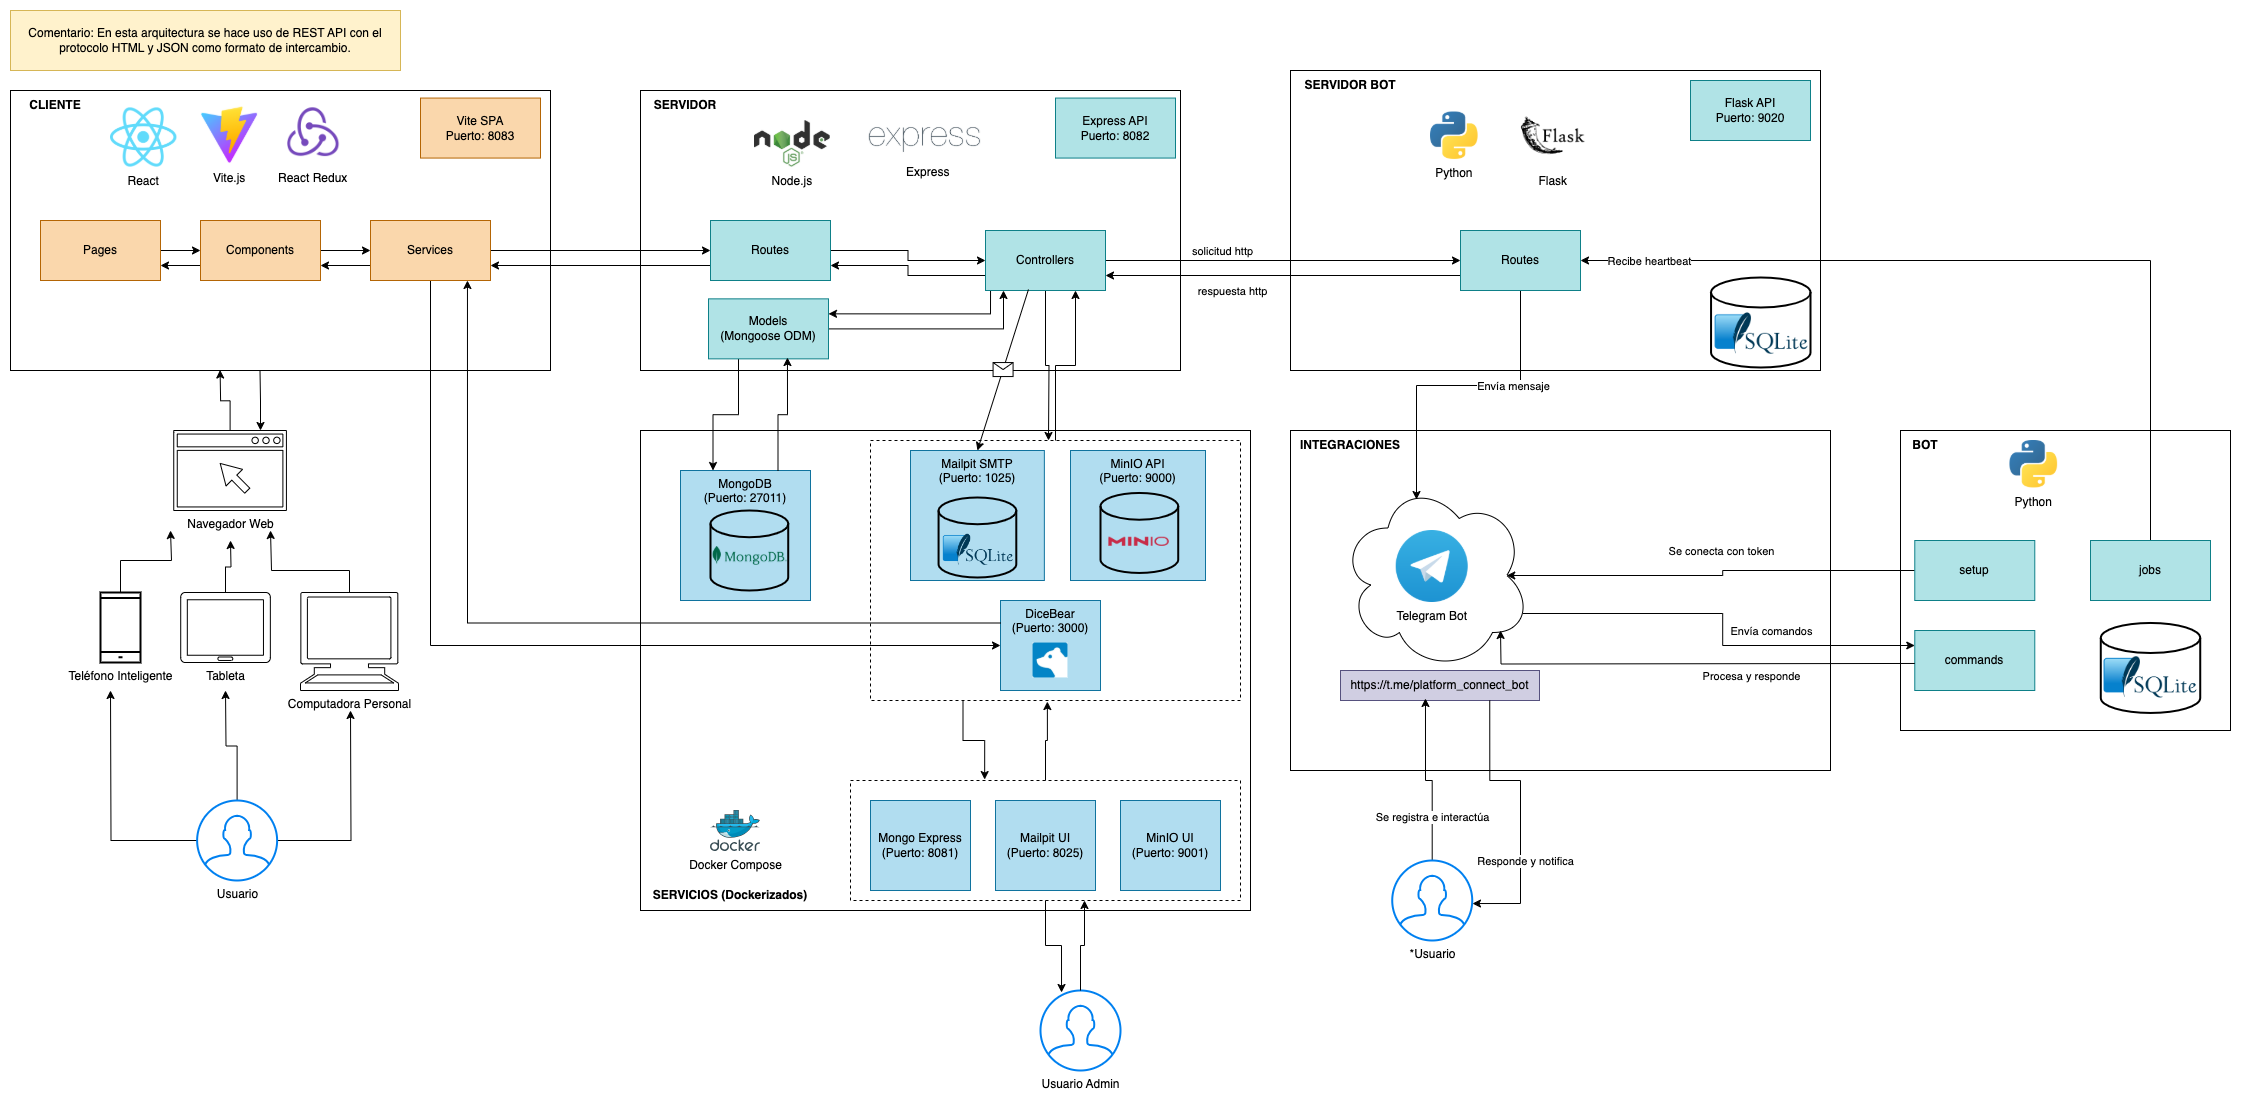
\includegraphics[width=\textwidth]{diagrama_arquitectura.png}
    \caption{Diagrama de Arquitectura}
    \label{fig:arquitectura}
\end{figure*}



\section{Resultados}
% Sección obligatoria.
% ¿Qué escribir en esta sección?
% Se hace un análisis de los resultados obtenidos. Esta sección contiene detalles acerca de cómo y por qué se obtuvieron dichos resultados. 
% Los resultados necesitan una descripción detallada de cómo fueron obtenidos (cuántos intentos, cuántas pruebas y cuántos casos exitosos).

El desarrollo de la solución web de capacitación empresarial basada en
microaprendizaje ha demostrado ser factible, cumpliendo con los objetivos
planteados en el diseño inicial. La plataforma implementa un sistema flexible
que facilita el acceso al aprendizaje y optimiza el tiempo de formación de los
empleados.

Como resultado, se han implementado módulos clave que permiten personalizar el
contenido educativo, garantizar accesibilidad desde múltiples dispositivos y
facilitar la interacción mediante plataformas externas. Uno de los aspectos
distintivos del sistema es la integración con Telegram, que mejora la
automatización de notificaciones para los usuarios.

Integrar el sistema de capacitación
con Telegram ha permitido ir optimizando la interacción y automatización de notificaciones para
los usuarios. A continuación, se presentan las principales pantallas que
demuestran esta funcionalidad.

\begin{figure}[htbp]
    \centering
    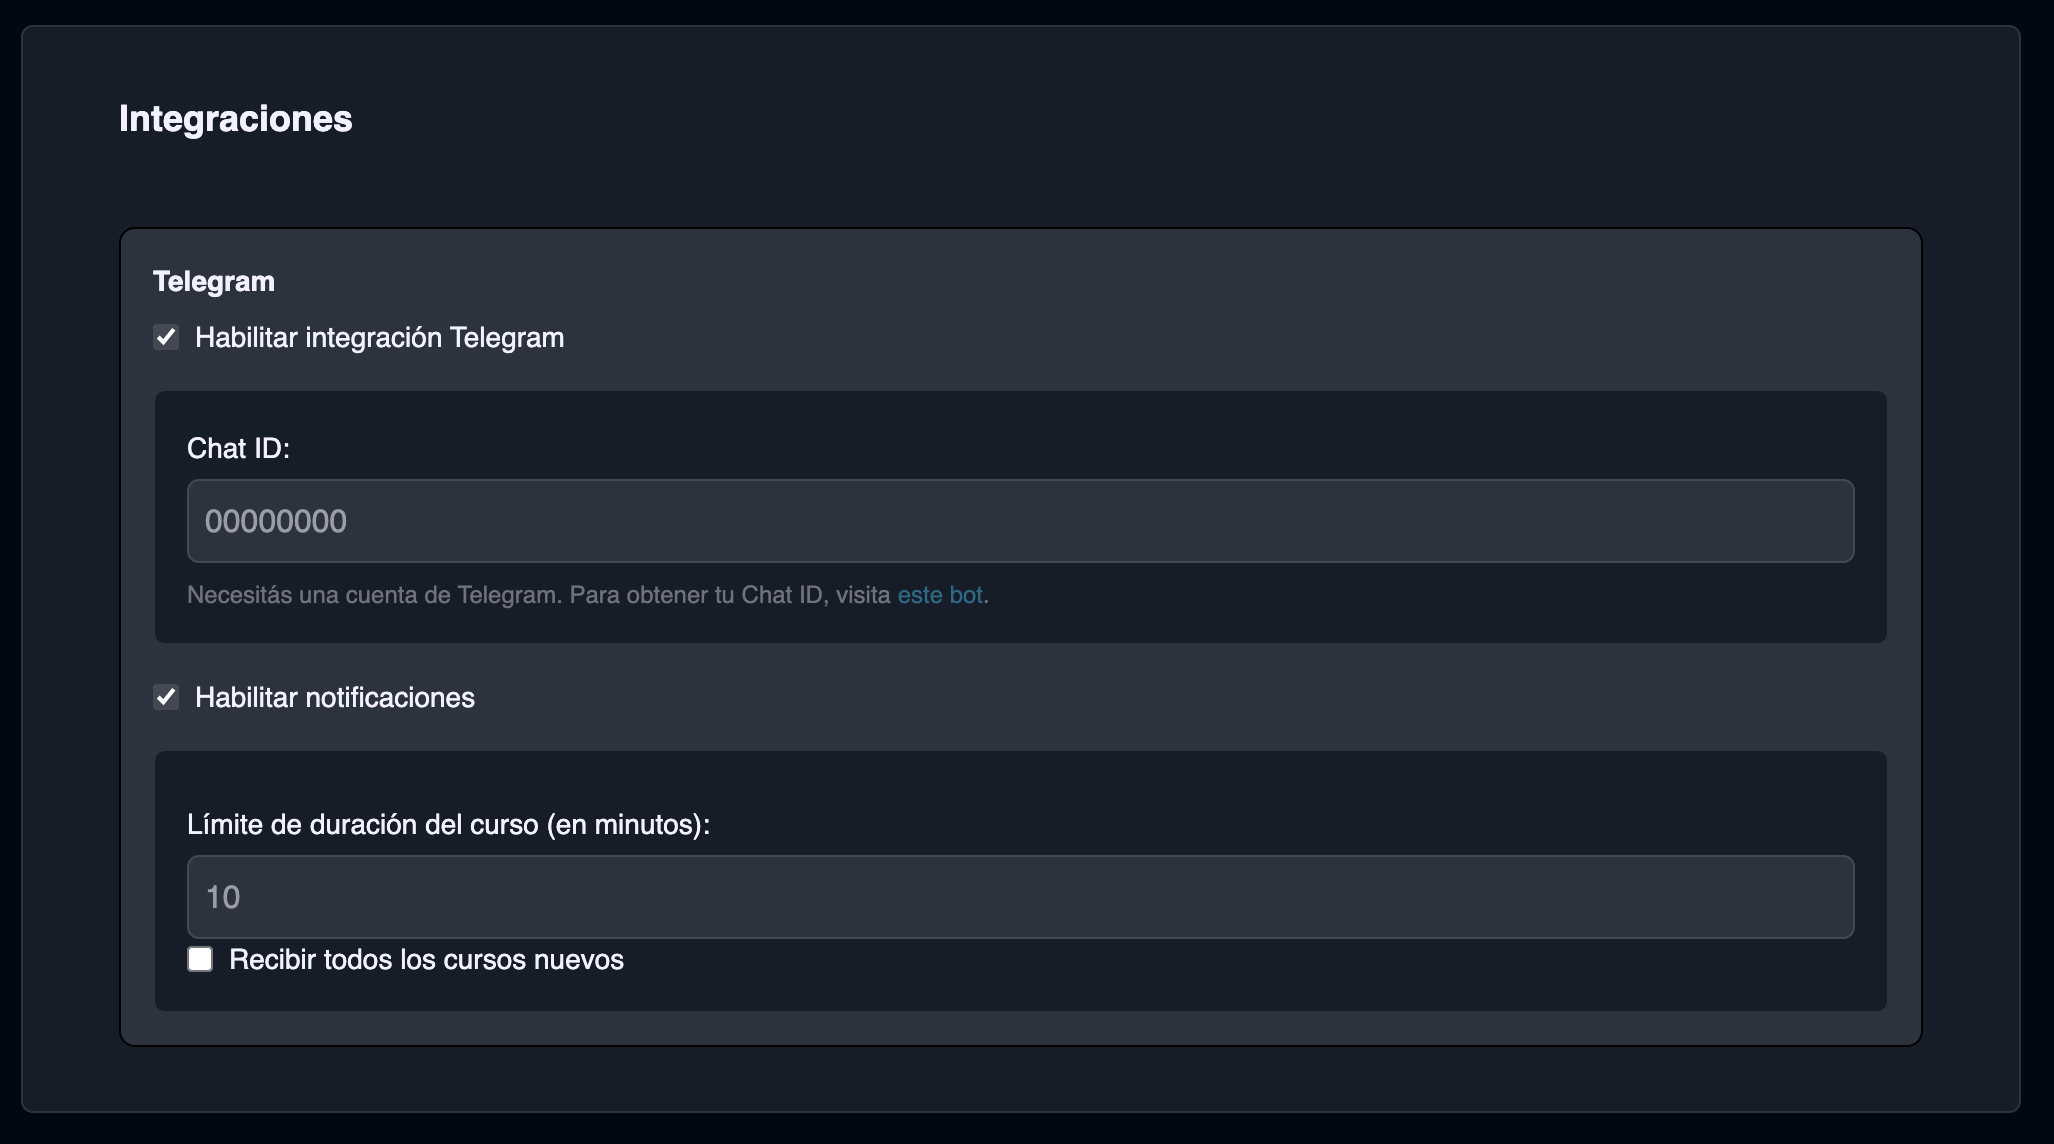
\includegraphics[width=\linewidth]{integracion_telegram/integracion_telegram_02.png}
    \caption{Interfaz del sistema con configuración de integración a Telegram}
    \label{fig:interfaz_integracion_telegram}
\end{figure}

La Figura \ref{fig:interfaz_integracion_telegram} muestra la sección del sistema
donde se encuentra la configuración para integrar Telegram. Desde esta interfaz,
los usuarios pueden activar la funcionalidad y gestionar sus preferencias de
notificación.

\begin{figure}[htbp]
    \centering
    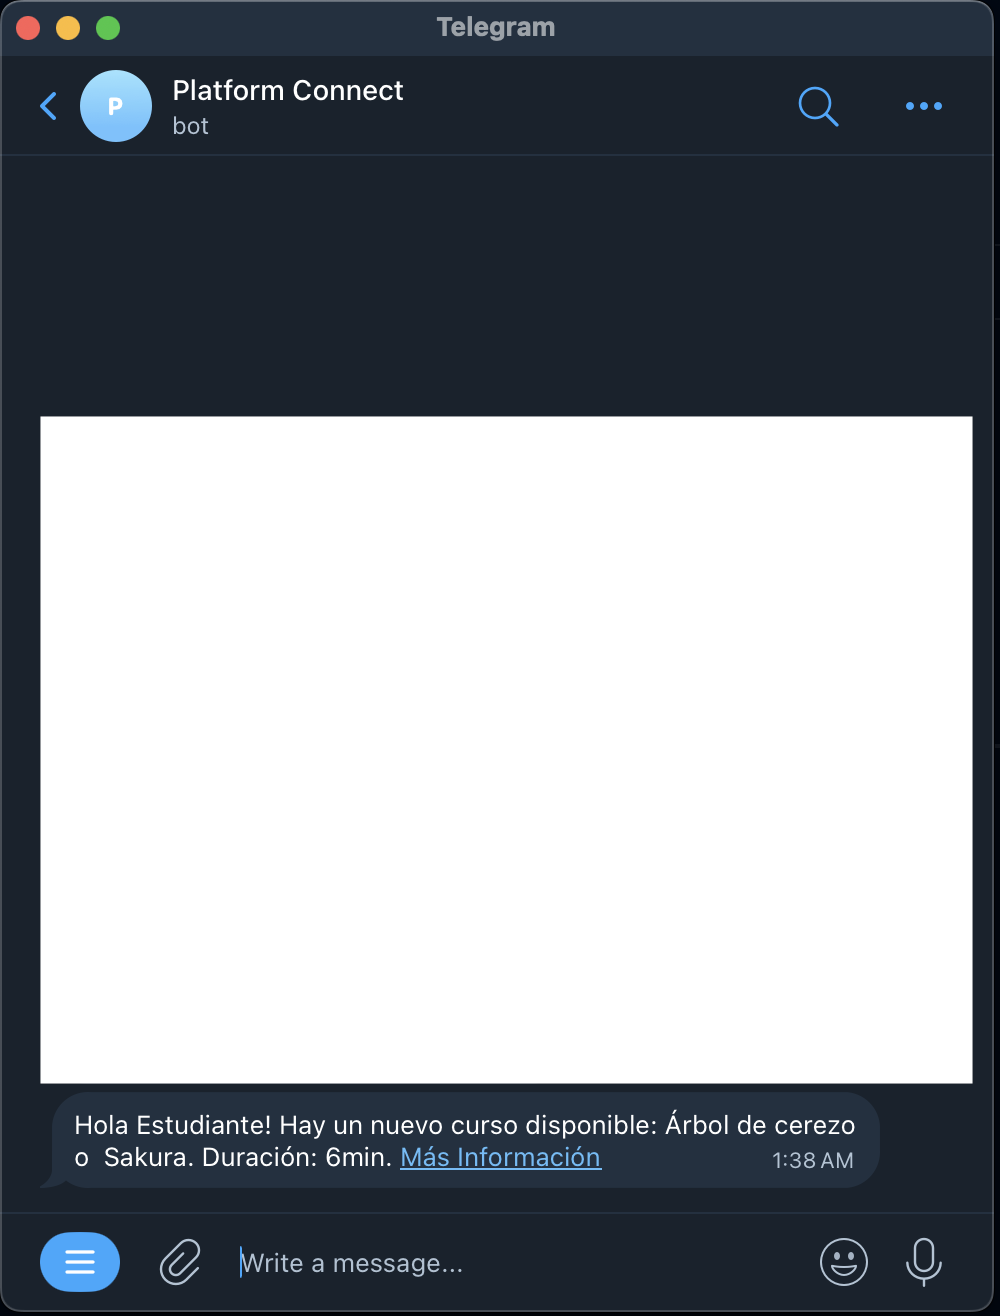
\includegraphics[width=\linewidth]{integracion_telegram/integracion_telegram_05.png}
    \caption{Notificación generada por el sistema en Telegram}
    \label{fig:notificacion_telegram}
\end{figure}

La Figura \ref{fig:notificacion_telegram} presenta una notificación enviada al
usuario a través de Telegram. Estas notificaciones permiten alertar sobre nuevos
cursos disponibles y recordatorios de formación, asegurando una comunicación
eficiente dentro del proceso de aprendizaje.

\begin{figure}[htbp]
    \centering
    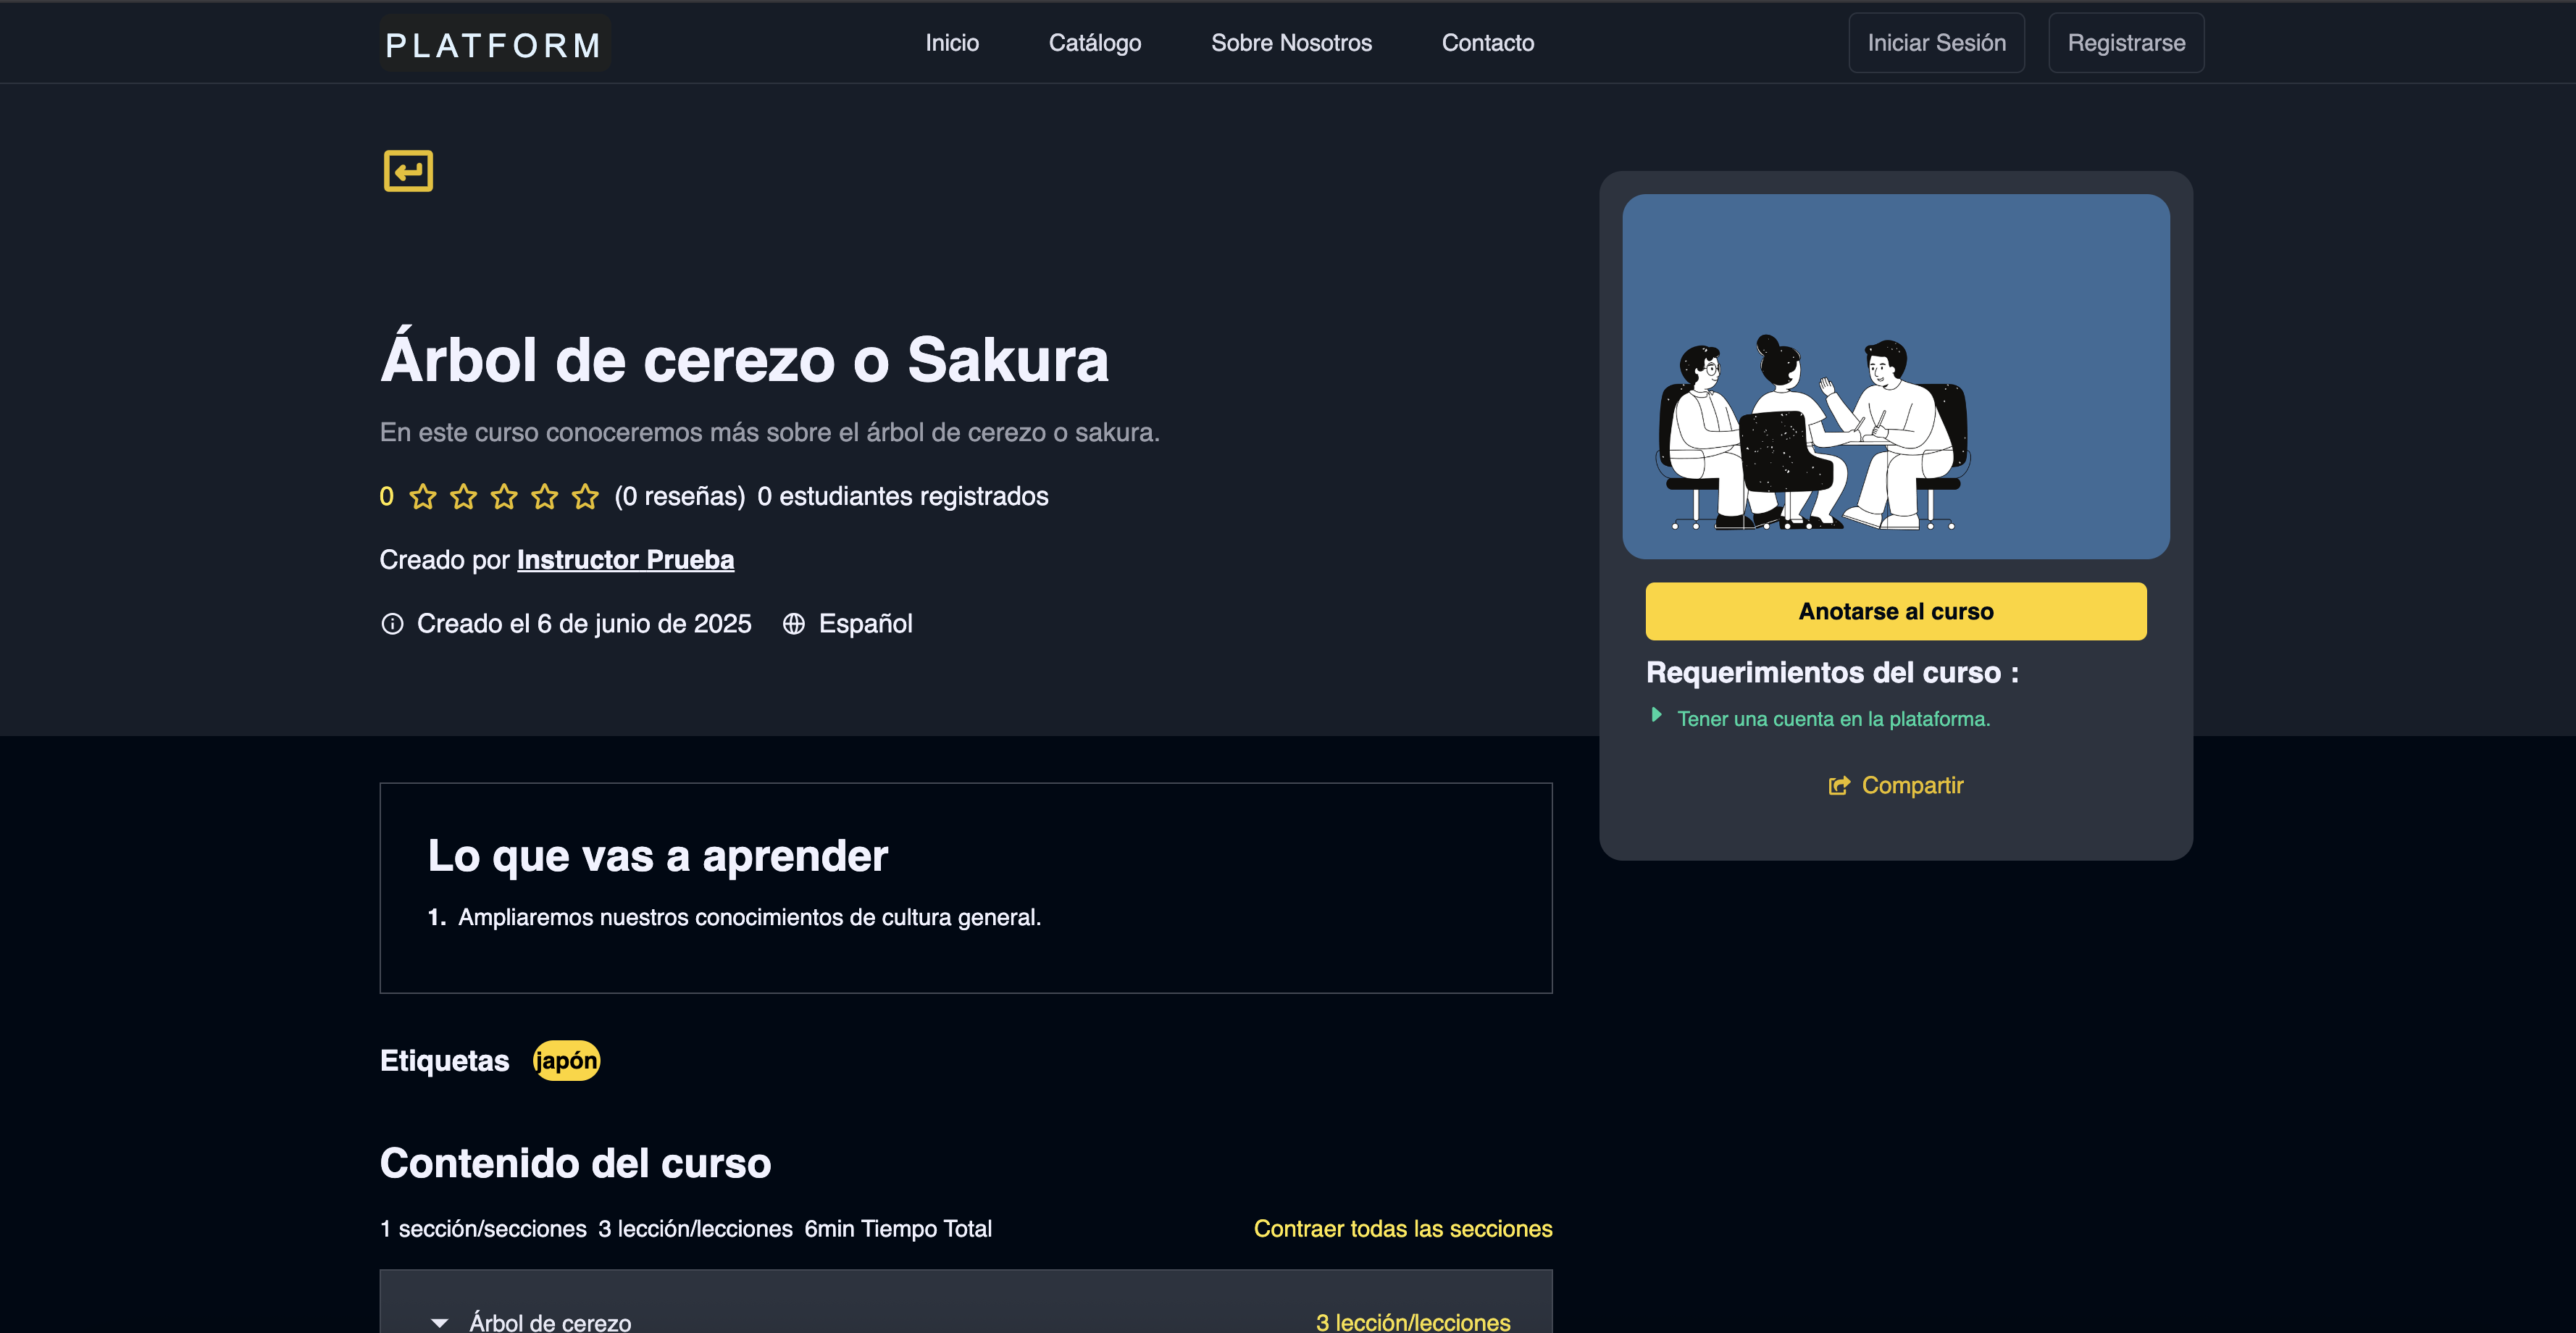
\includegraphics[width=\linewidth]{plataforma/plataforma_07.png}
    \caption{Interfaz del sistema tras acceder desde la notificación}
    \label{fig:interfaz_curso_ejemplo}
\end{figure}

La Figura \ref{fig:interfaz_curso_ejemplo} muestra la vista de un curso al que
el usuario accede tras hacer clic en la notificación recibida en Telegram. Desde
esta pantalla, el usuario puede explorar los detalles del curso y realizar su
inscripción de manera rápida, garantizando una transición fluida entre la
plataforma de mensajería y el sistema de capacitación.

Los principales logros de la solución incluyen:
\begin{itemize}
    \item Personalización del contenido educativo según el perfil y objetivos
    individuales de los empleados.
    \item Integración con plataformas de mensajería para optimizar la
    interacción y accesibilidad.
    \item Accesibilidad multiplataforma, permitiendo el uso desde dispositivos
    móviles y de escritorio.
\end{itemize}

Esto demuestra por un lado la viabilidad del sistema y su capacidad de
adaptación a diversos entornos de capacitación empresarial. Por otro lado, estos
resultados reflejan la integración efectiva del sistema con plataformas
externas, mejorando la accesibilidad y optimizando la experiencia del usuario en
el proceso de aprendizaje.


\section{Conclusión}
\blindtext

\appendices
% Este apéndice proporciona información complementaria para reforzar la solución
% propuesta sin sobrecargar el cuerpo principal del paper.
% - Especificaciones de software y hardware requeridas.
% - Diagramas de arquitectura del sistema LMS.
% - Algoritmos utilizados para personalizar el microaprendizaje.
% - Capturas de pantalla o ejemplos de la interfaz del LMS.
% - Resultados detallados de pruebas piloto o estudios de usabilidad.
% - Comparación con otros LMS tradicionales y sus limitaciones.
% - Formularios utilizados para evaluar la efectividad del sistema.
% - Respuestas clave de usuarios o docentes sobre la experiencia de aprendizaje.
% - Segmentos relevantes del código para la implementación del LMS.
% - Scripts utilizados para la automatización de contenido microlearning.
% - Fórmulas aplicadas en la recomendación de contenidos.
% - Estadísticas detalladas sobre mejora en el aprendizaje.
% - Glosario de términos técnicos utilizados.
% - Documentación técnica adicional.

% La opción [H] en \begin{figure}[H] proviene del paquete float y significa ''Colocar la figura exactamente aquí''.

\appendices
\section{Interfaz del Sistema en Imágenes}

\begin{figure}[H]
    \centering
    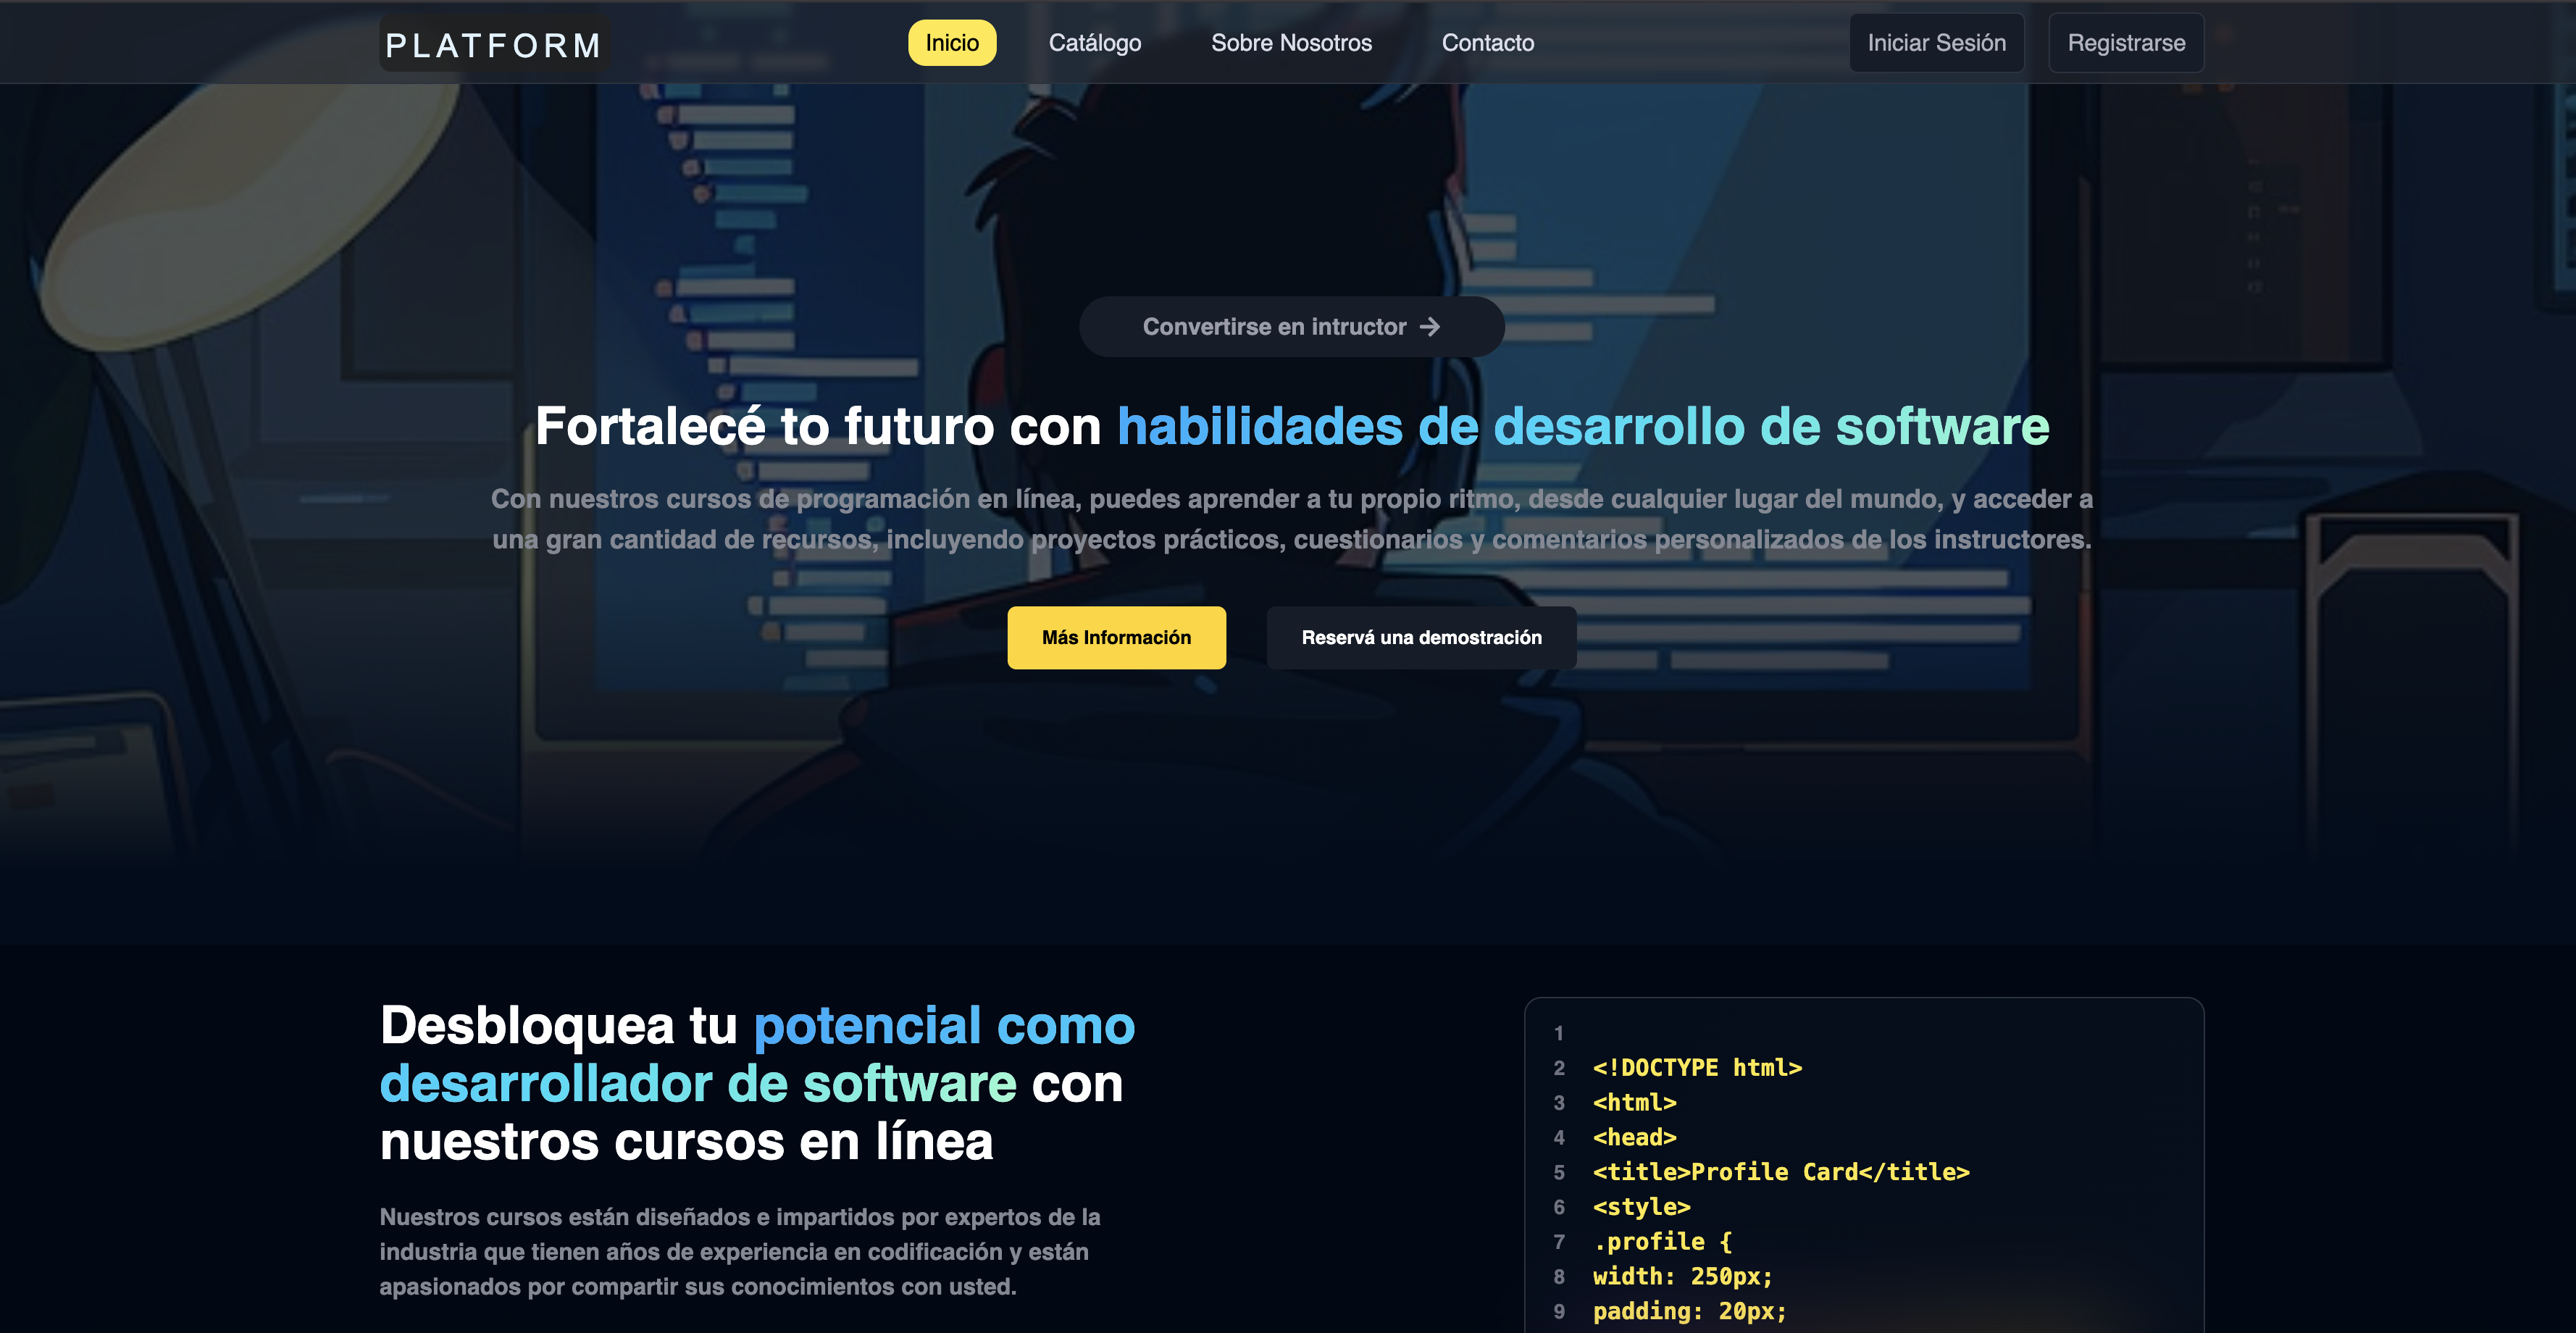
\includegraphics[width=\linewidth]{plataforma/plataforma_01.png}
    \caption{Interfaz de la página de inicio}
    \label{fig:interfaz_sistema_pagina_inicio}
\end{figure}

\begin{figure}[H]
    \centering
    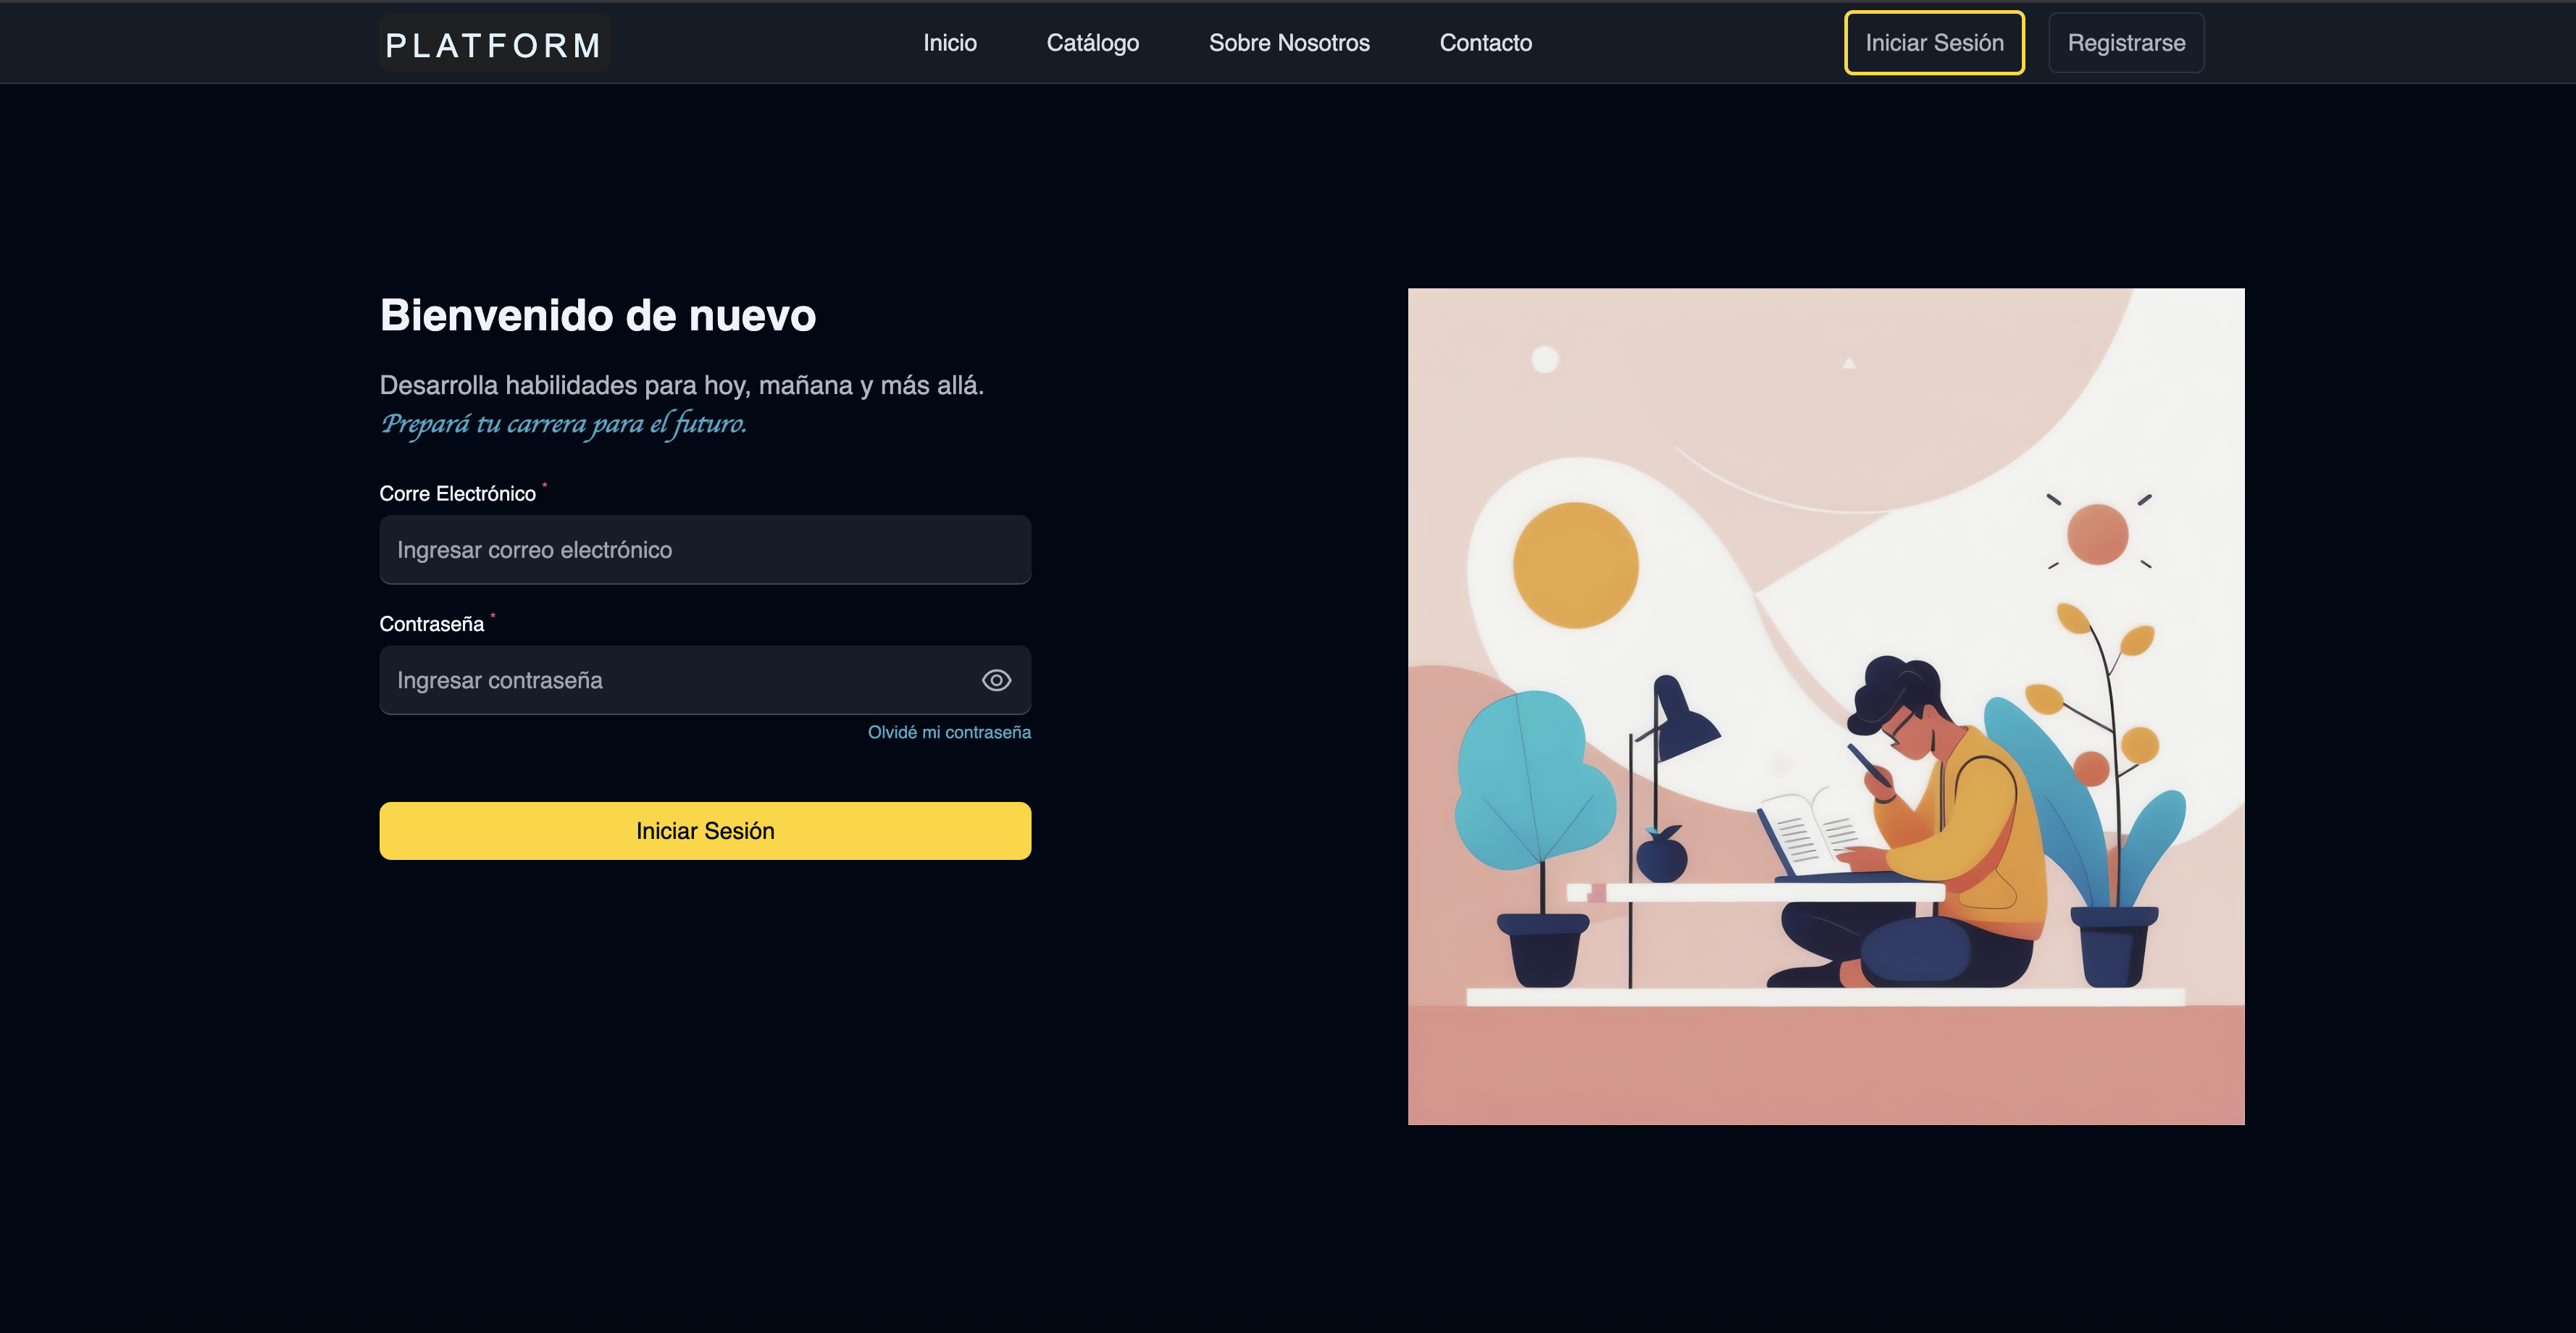
\includegraphics[width=\linewidth]{plataforma/plataforma_02.png}
    \caption{Interfaz de inicio de sesión}
    \label{fig:interfaz_sistema_inicio_sesión}
\end{figure}

\begin{figure}[H]
    \centering
    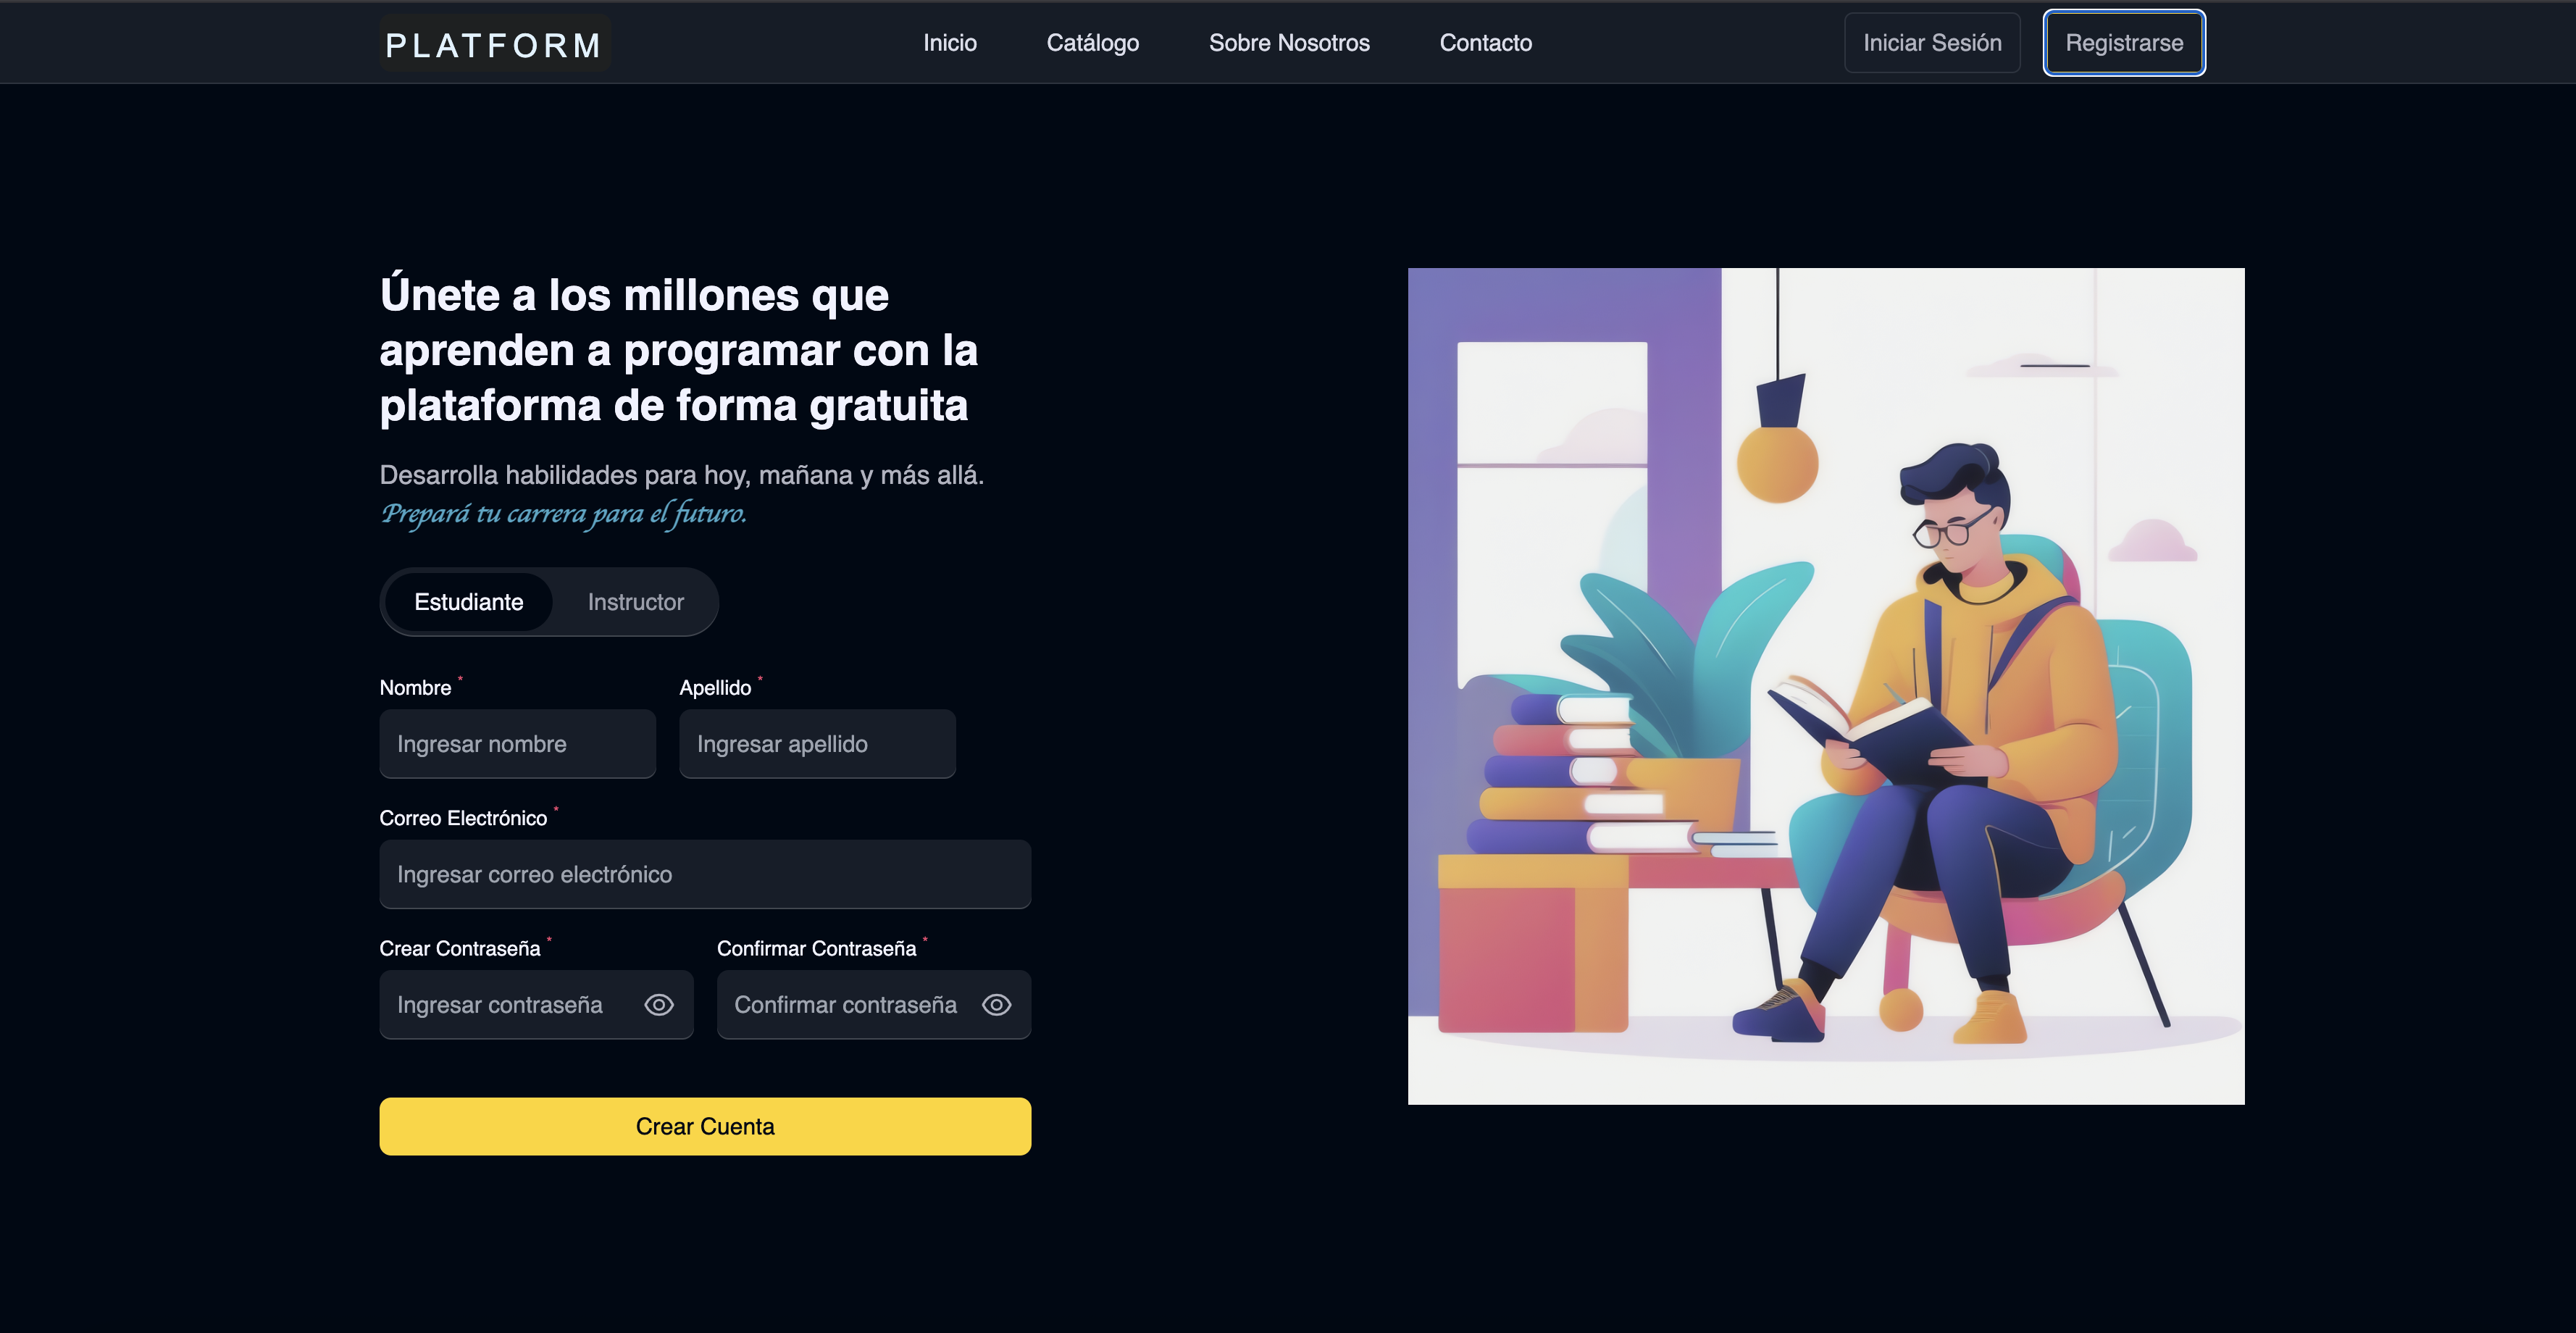
\includegraphics[width=\linewidth]{plataforma/plataforma_03.png}
    \caption{Interfaz del registro de usuario}
    \label{fig:interfaz_sistema_registro_usuario}
\end{figure}

\begin{figure}[H]
    \centering
    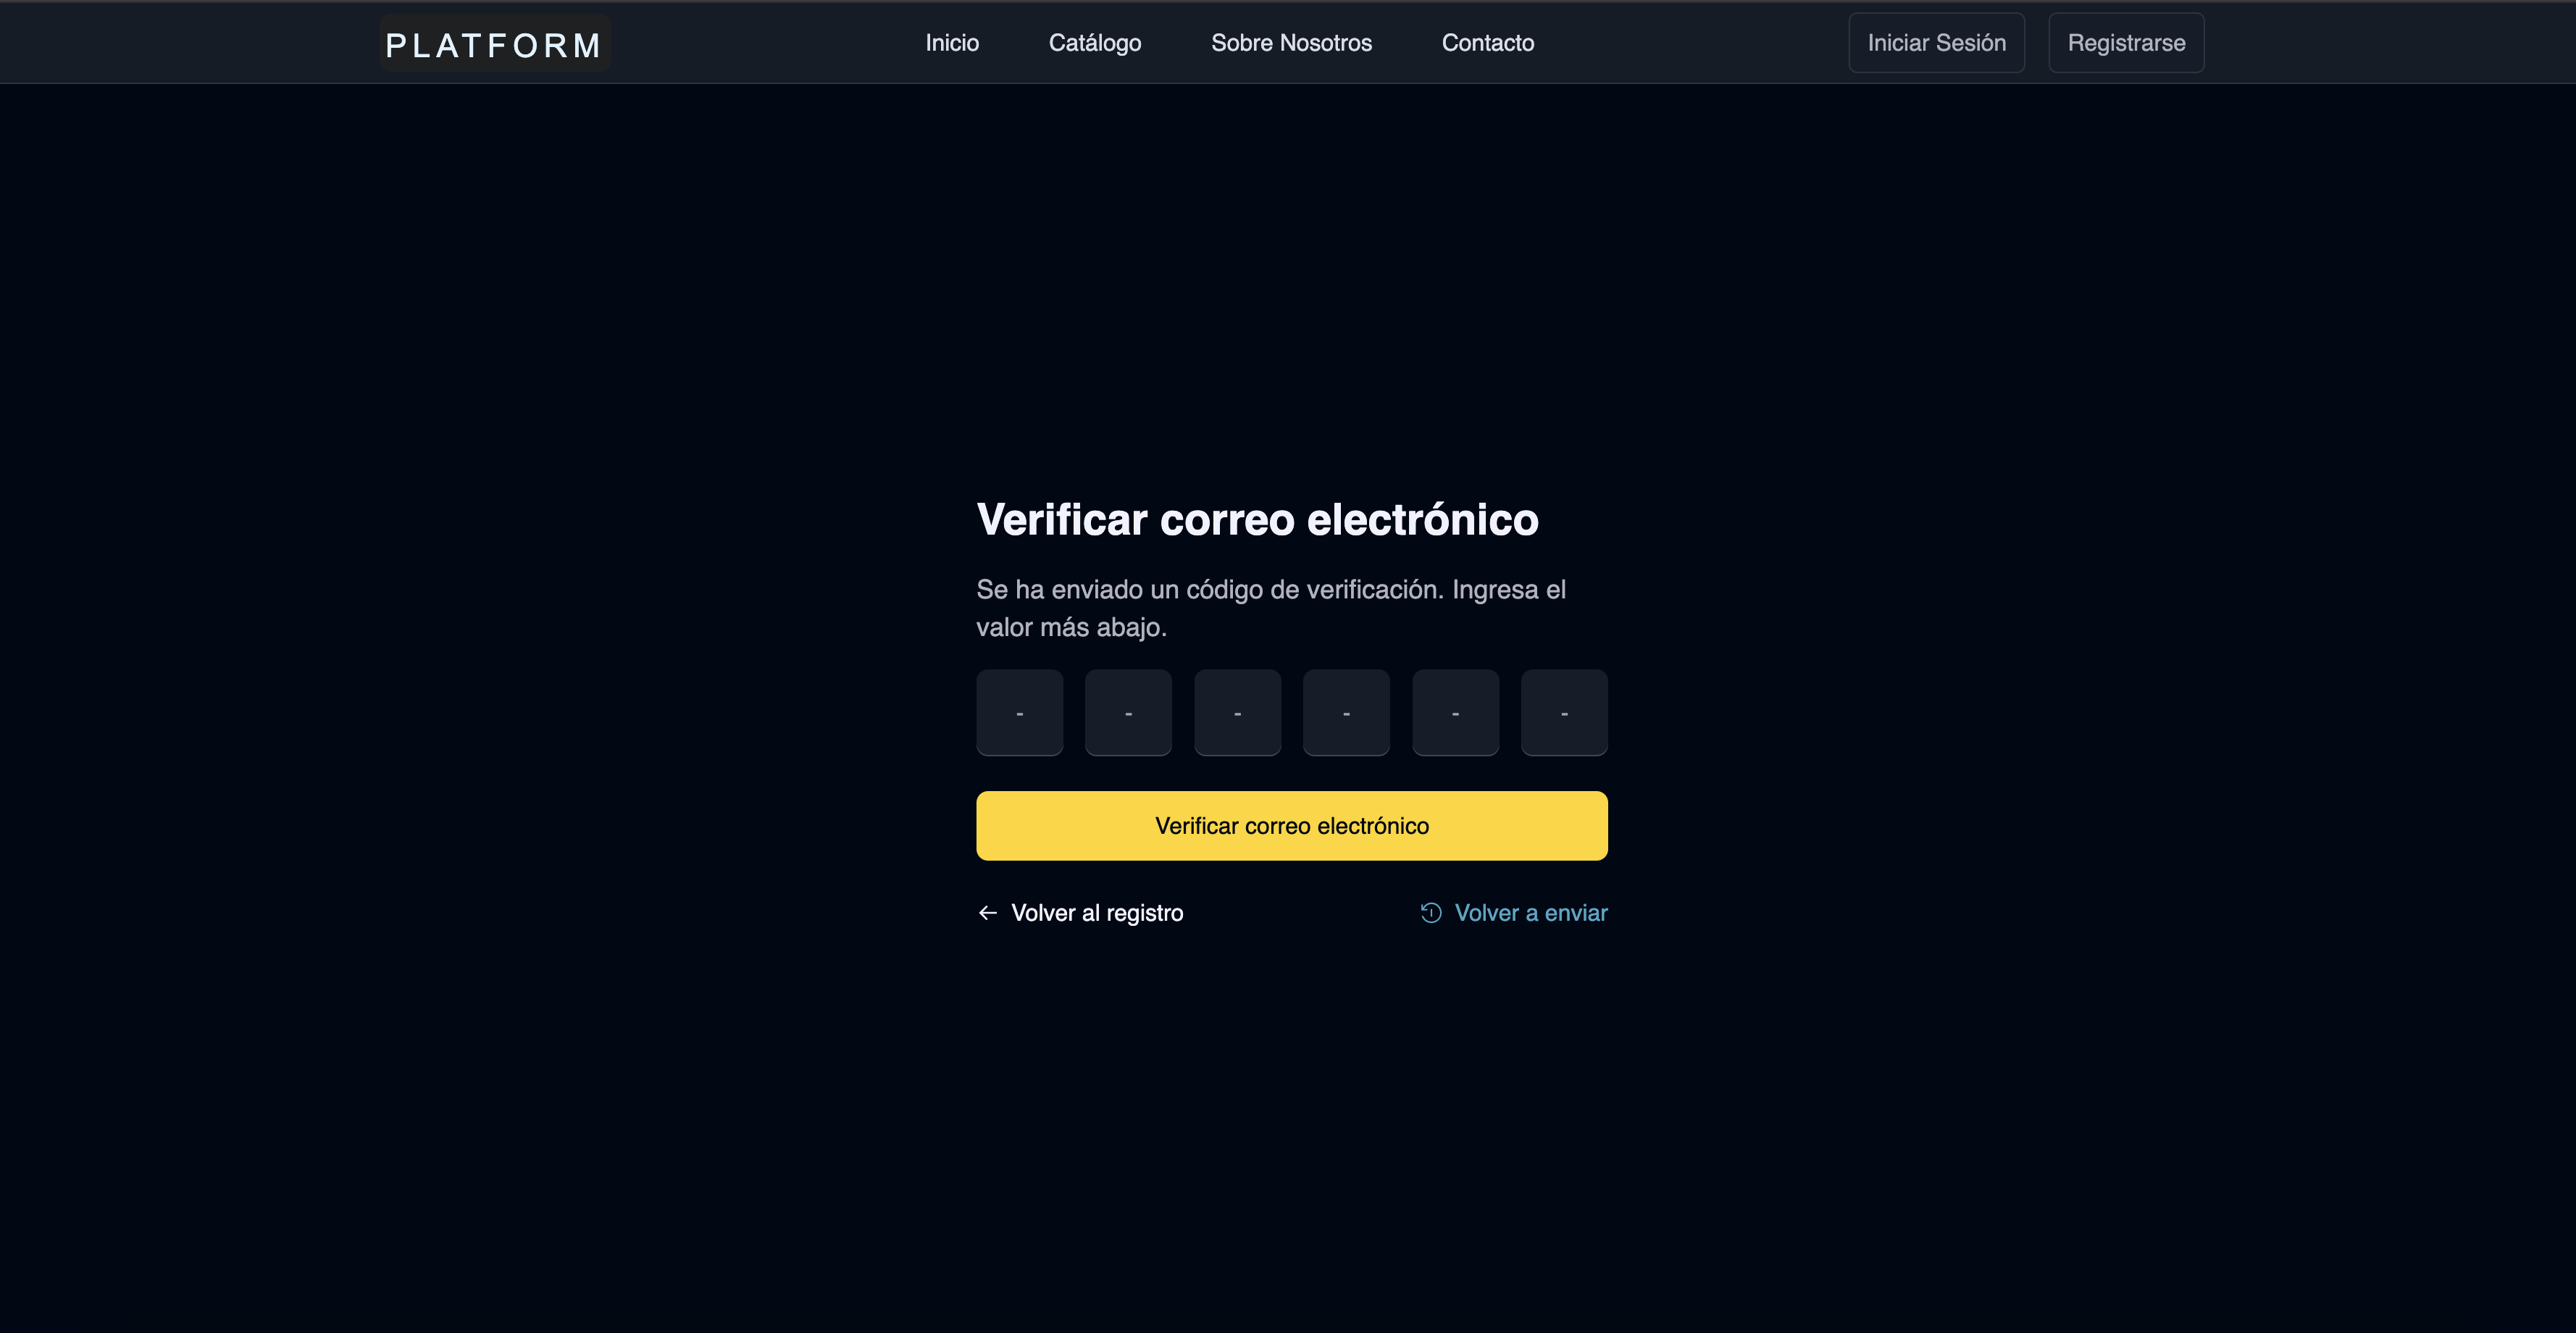
\includegraphics[width=\linewidth]{plataforma/plataforma_04.png}
    \caption{Interfaz de verificar correo}
    \label{fig:interfaz_sistema_verificar_correo}
\end{figure}

\begin{figure}[H]
    \centering
    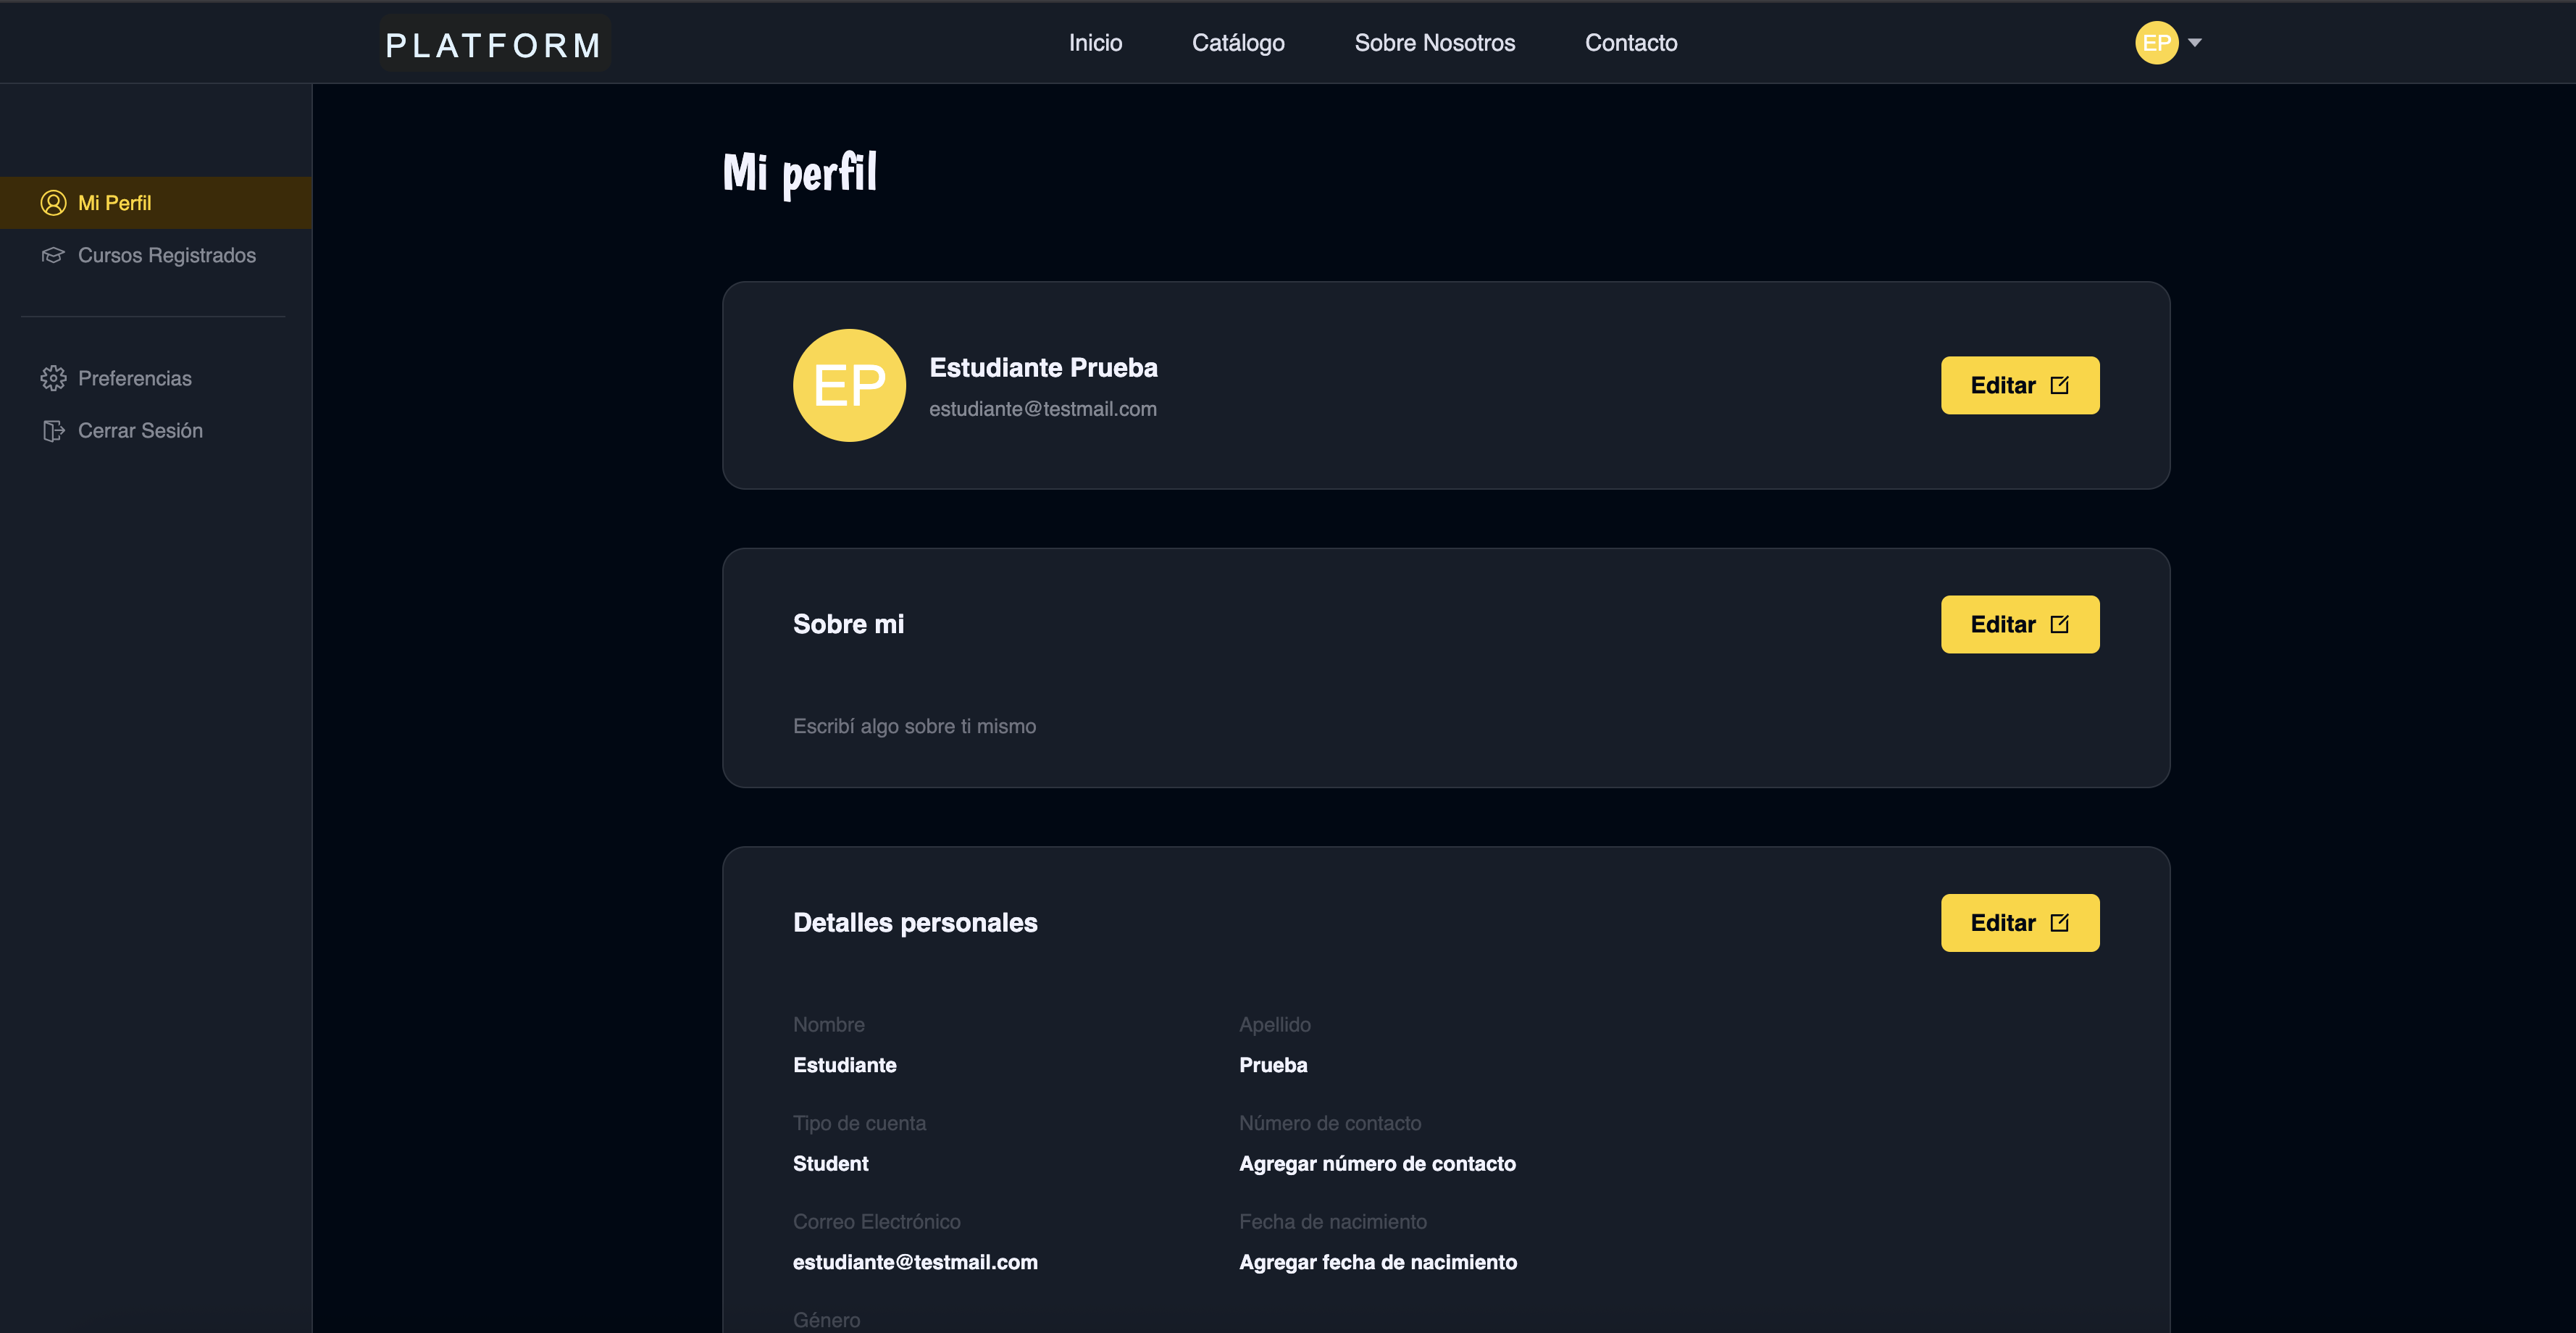
\includegraphics[width=\linewidth]{plataforma/plataforma_05.png}
    \caption{Interfaz de perfil de usuario}
    \label{fig:interfaz_sistema_perfil_usuario}
\end{figure}

\begin{figure}[H]
    \centering
    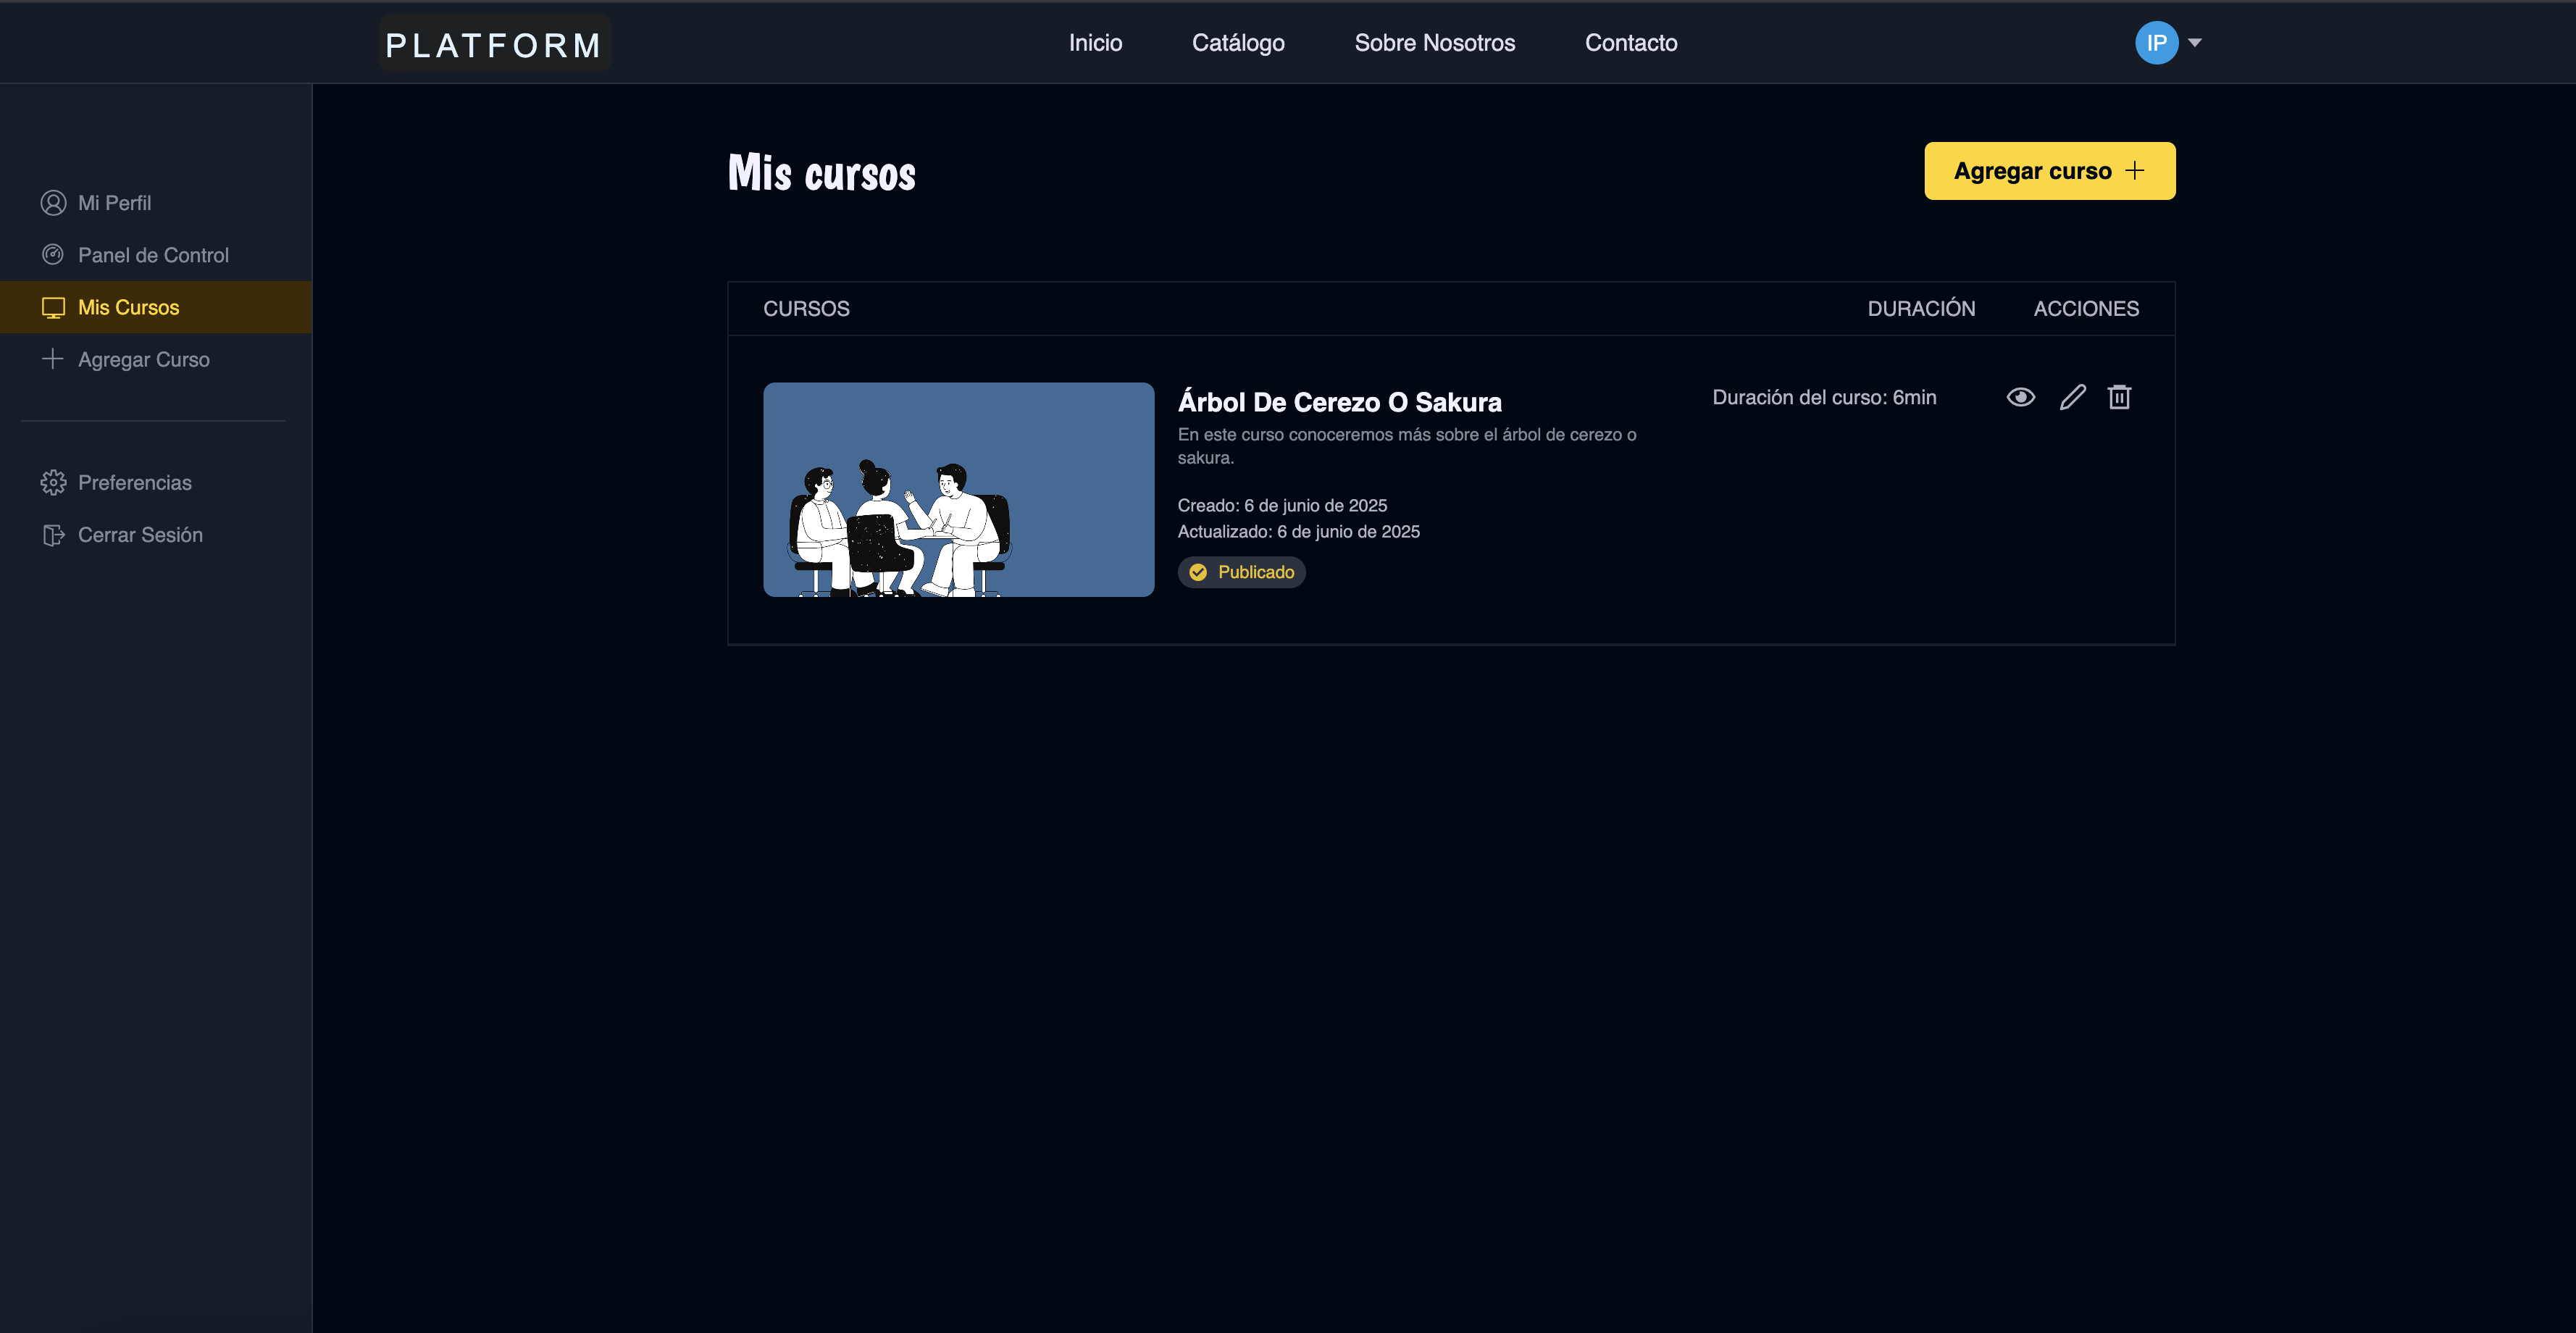
\includegraphics[width=\linewidth]{plataforma/plataforma_06.png}
    \caption{Interfaz de cursos usuario instructor}
    \label{fig:interfaz_sistema_cursos_usuario_instructor}
\end{figure}

\begin{figure}[H]
    \centering
    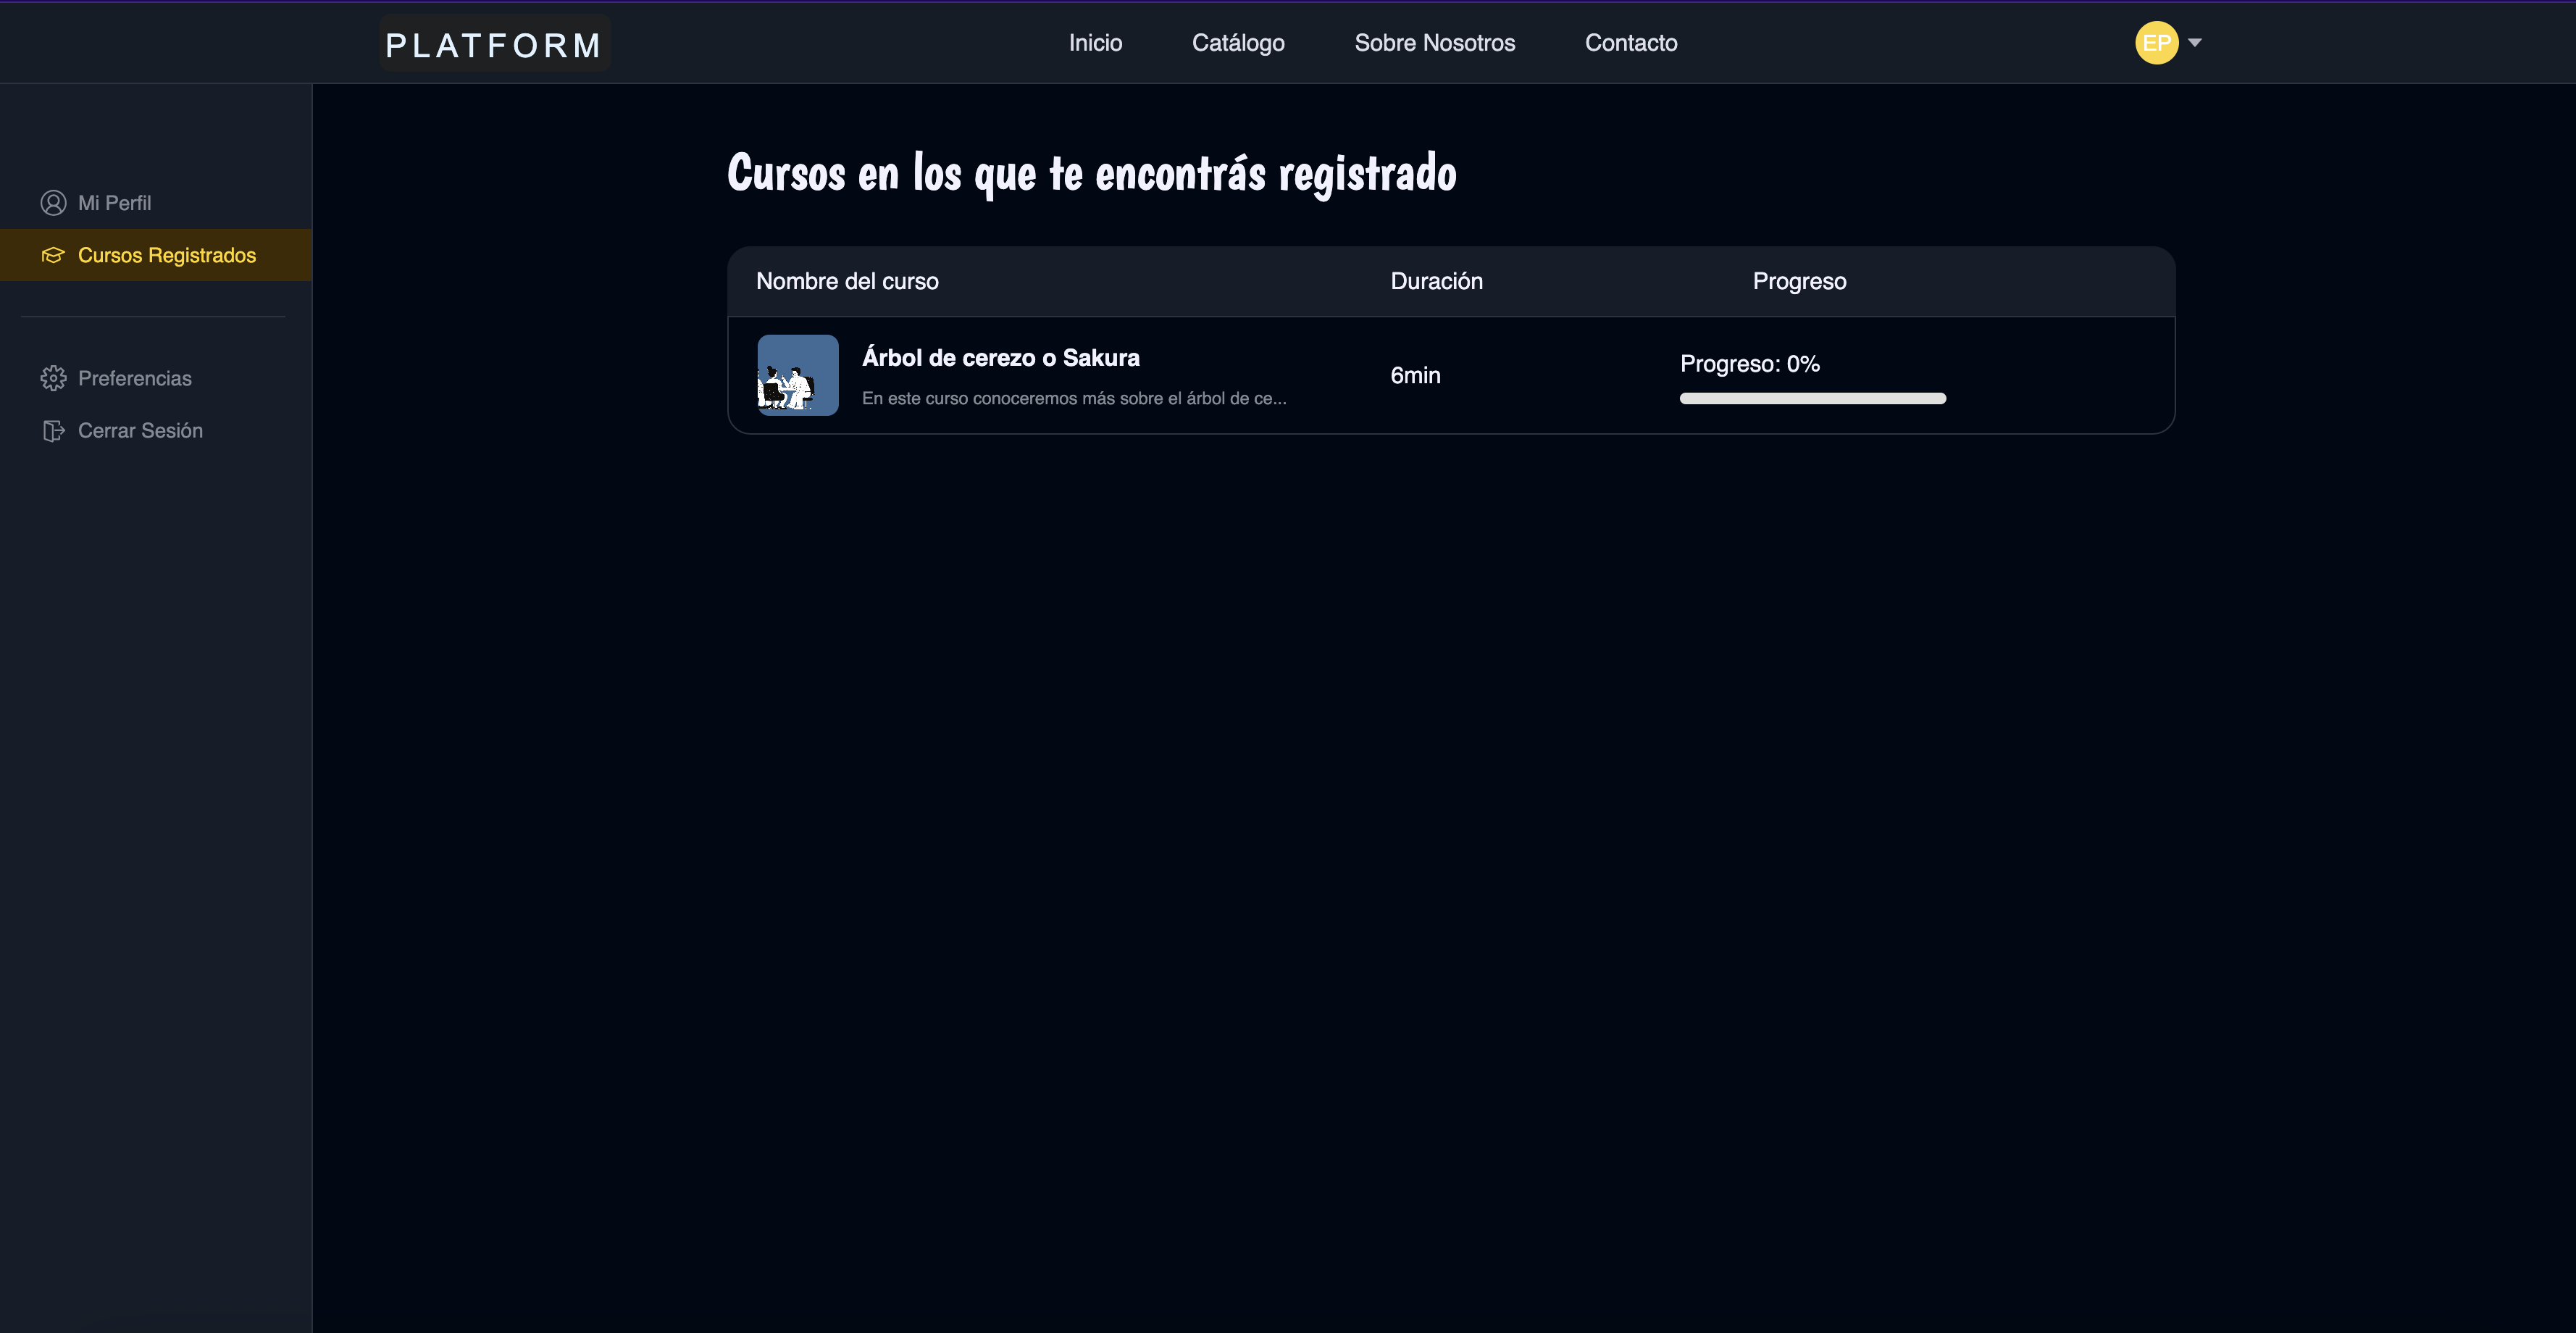
\includegraphics[width=\linewidth]{plataforma/plataforma_08.png}
    \caption{Interfaz de cursos usuario estudiante}
    \label{fig:interfaz_sistema_cursos_usuario_estudiante}
\end{figure}


\section{Lecciones en Imágenes}

\begin{figure}[H]
    \centering
    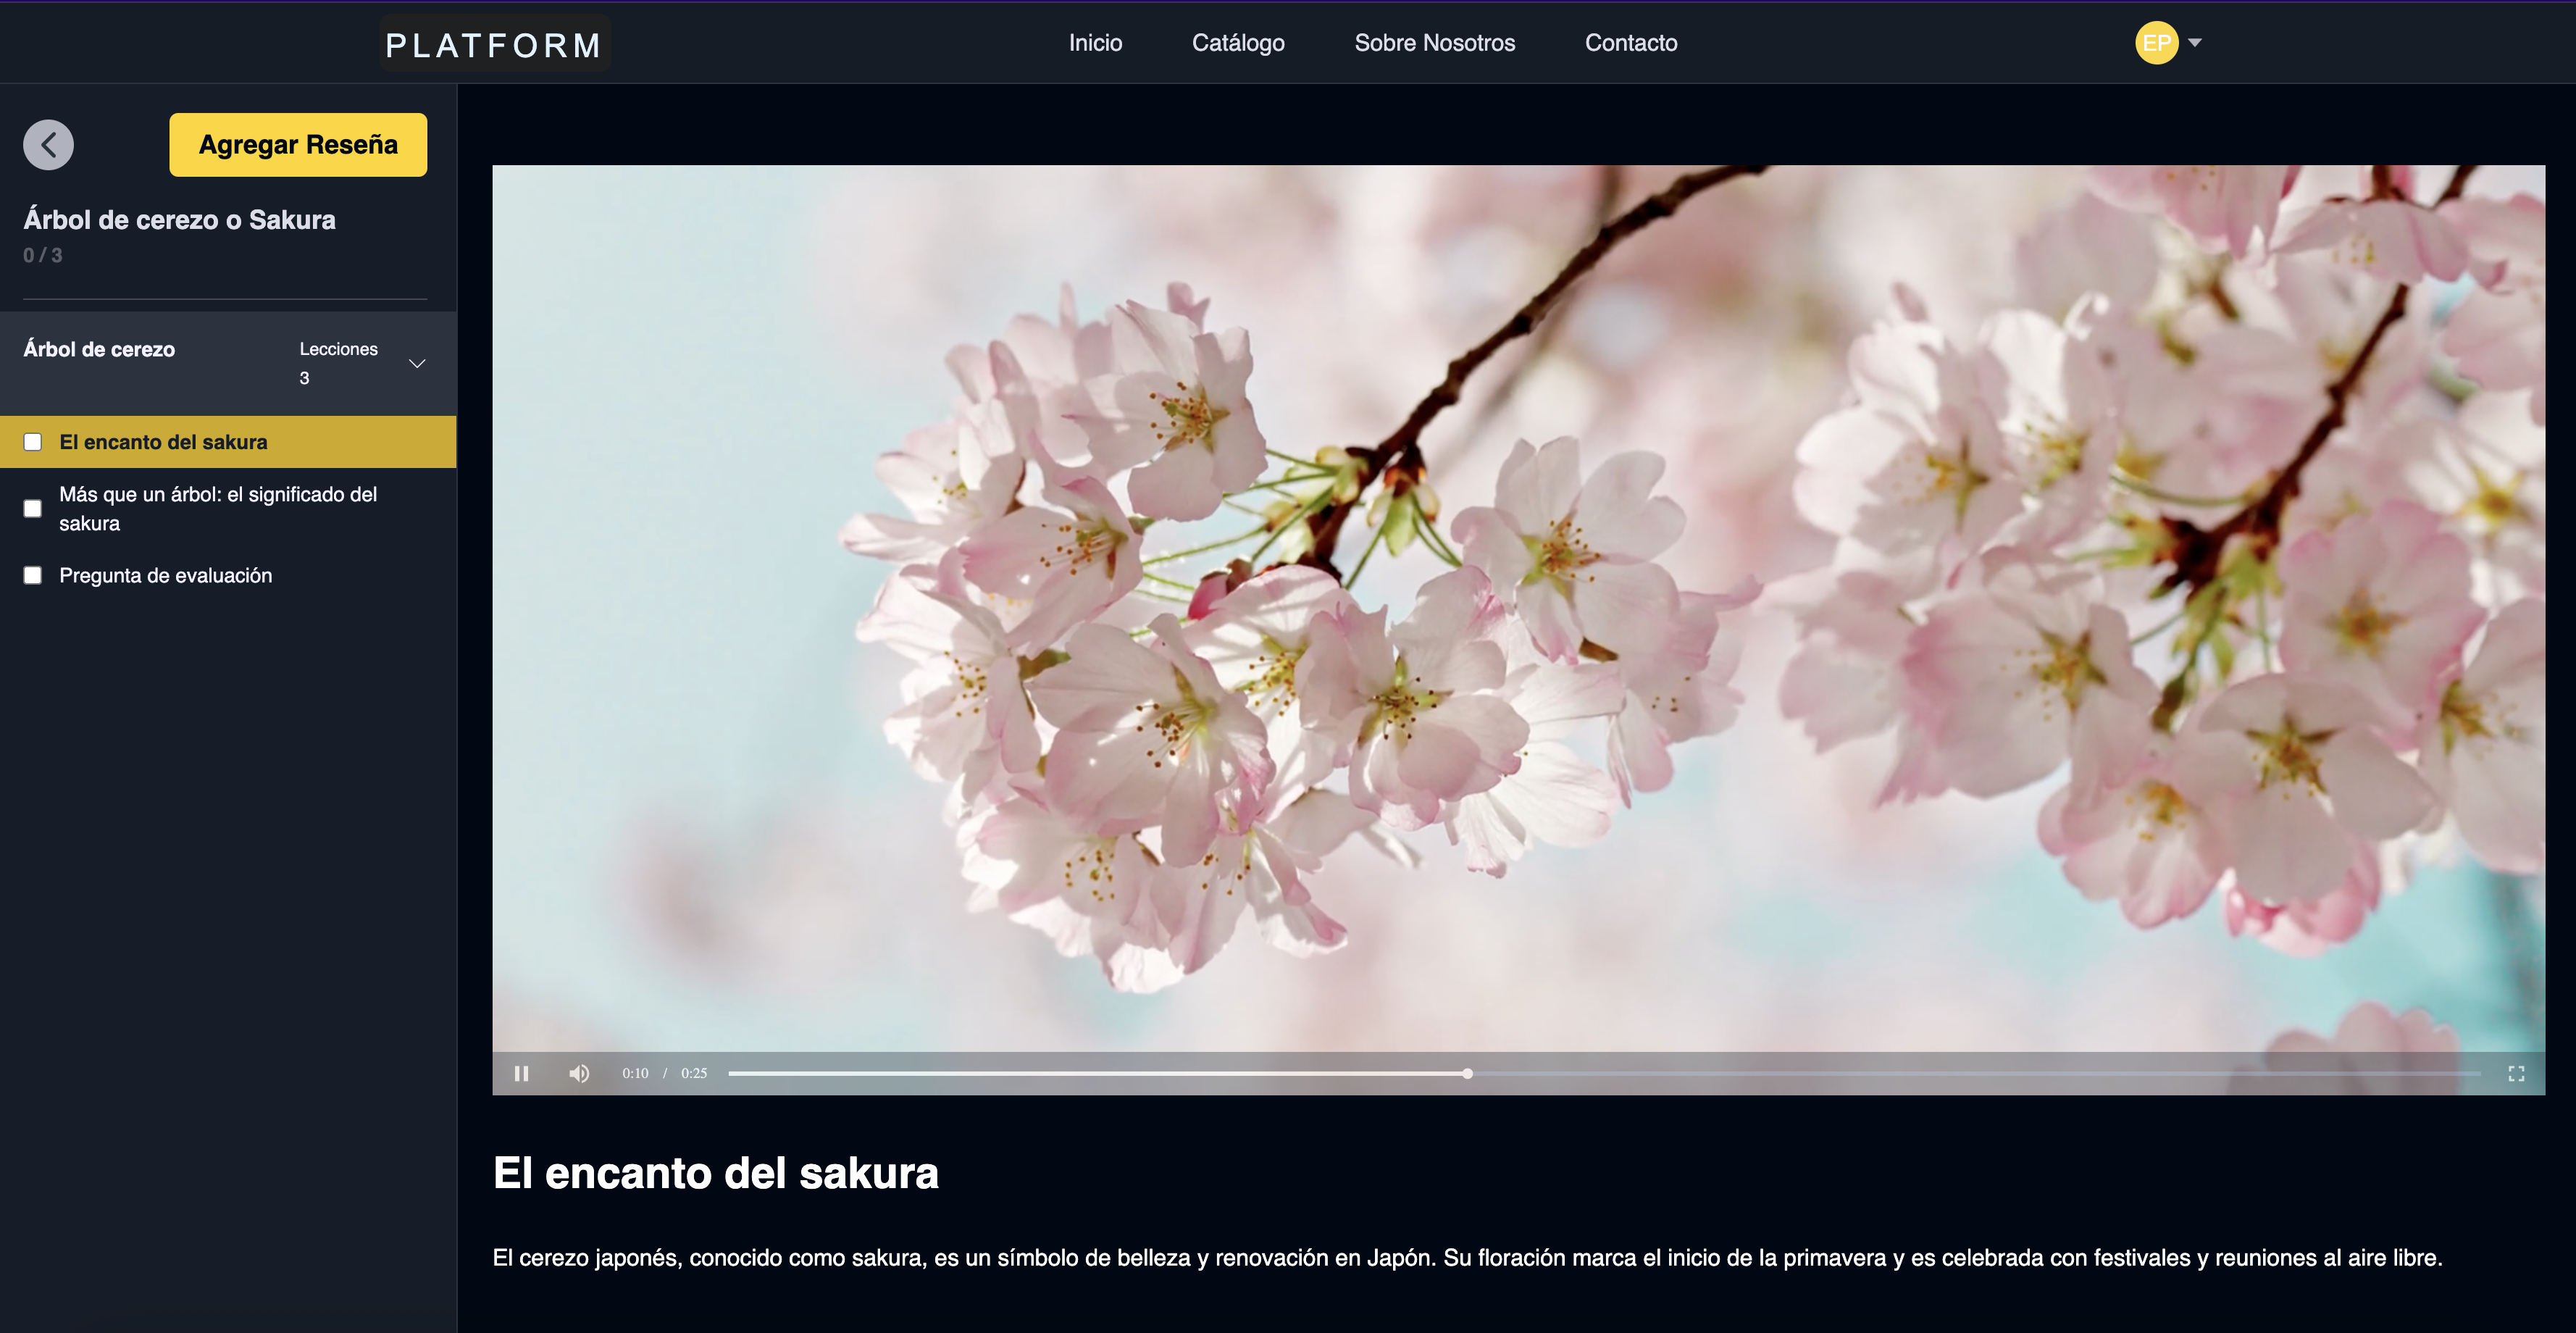
\includegraphics[width=\linewidth]{leccion/leccion_01.png}
    \caption{Lección tipo video}
    \label{fig:leccion_video}
\end{figure}

\begin{figure}[H]
    \centering
    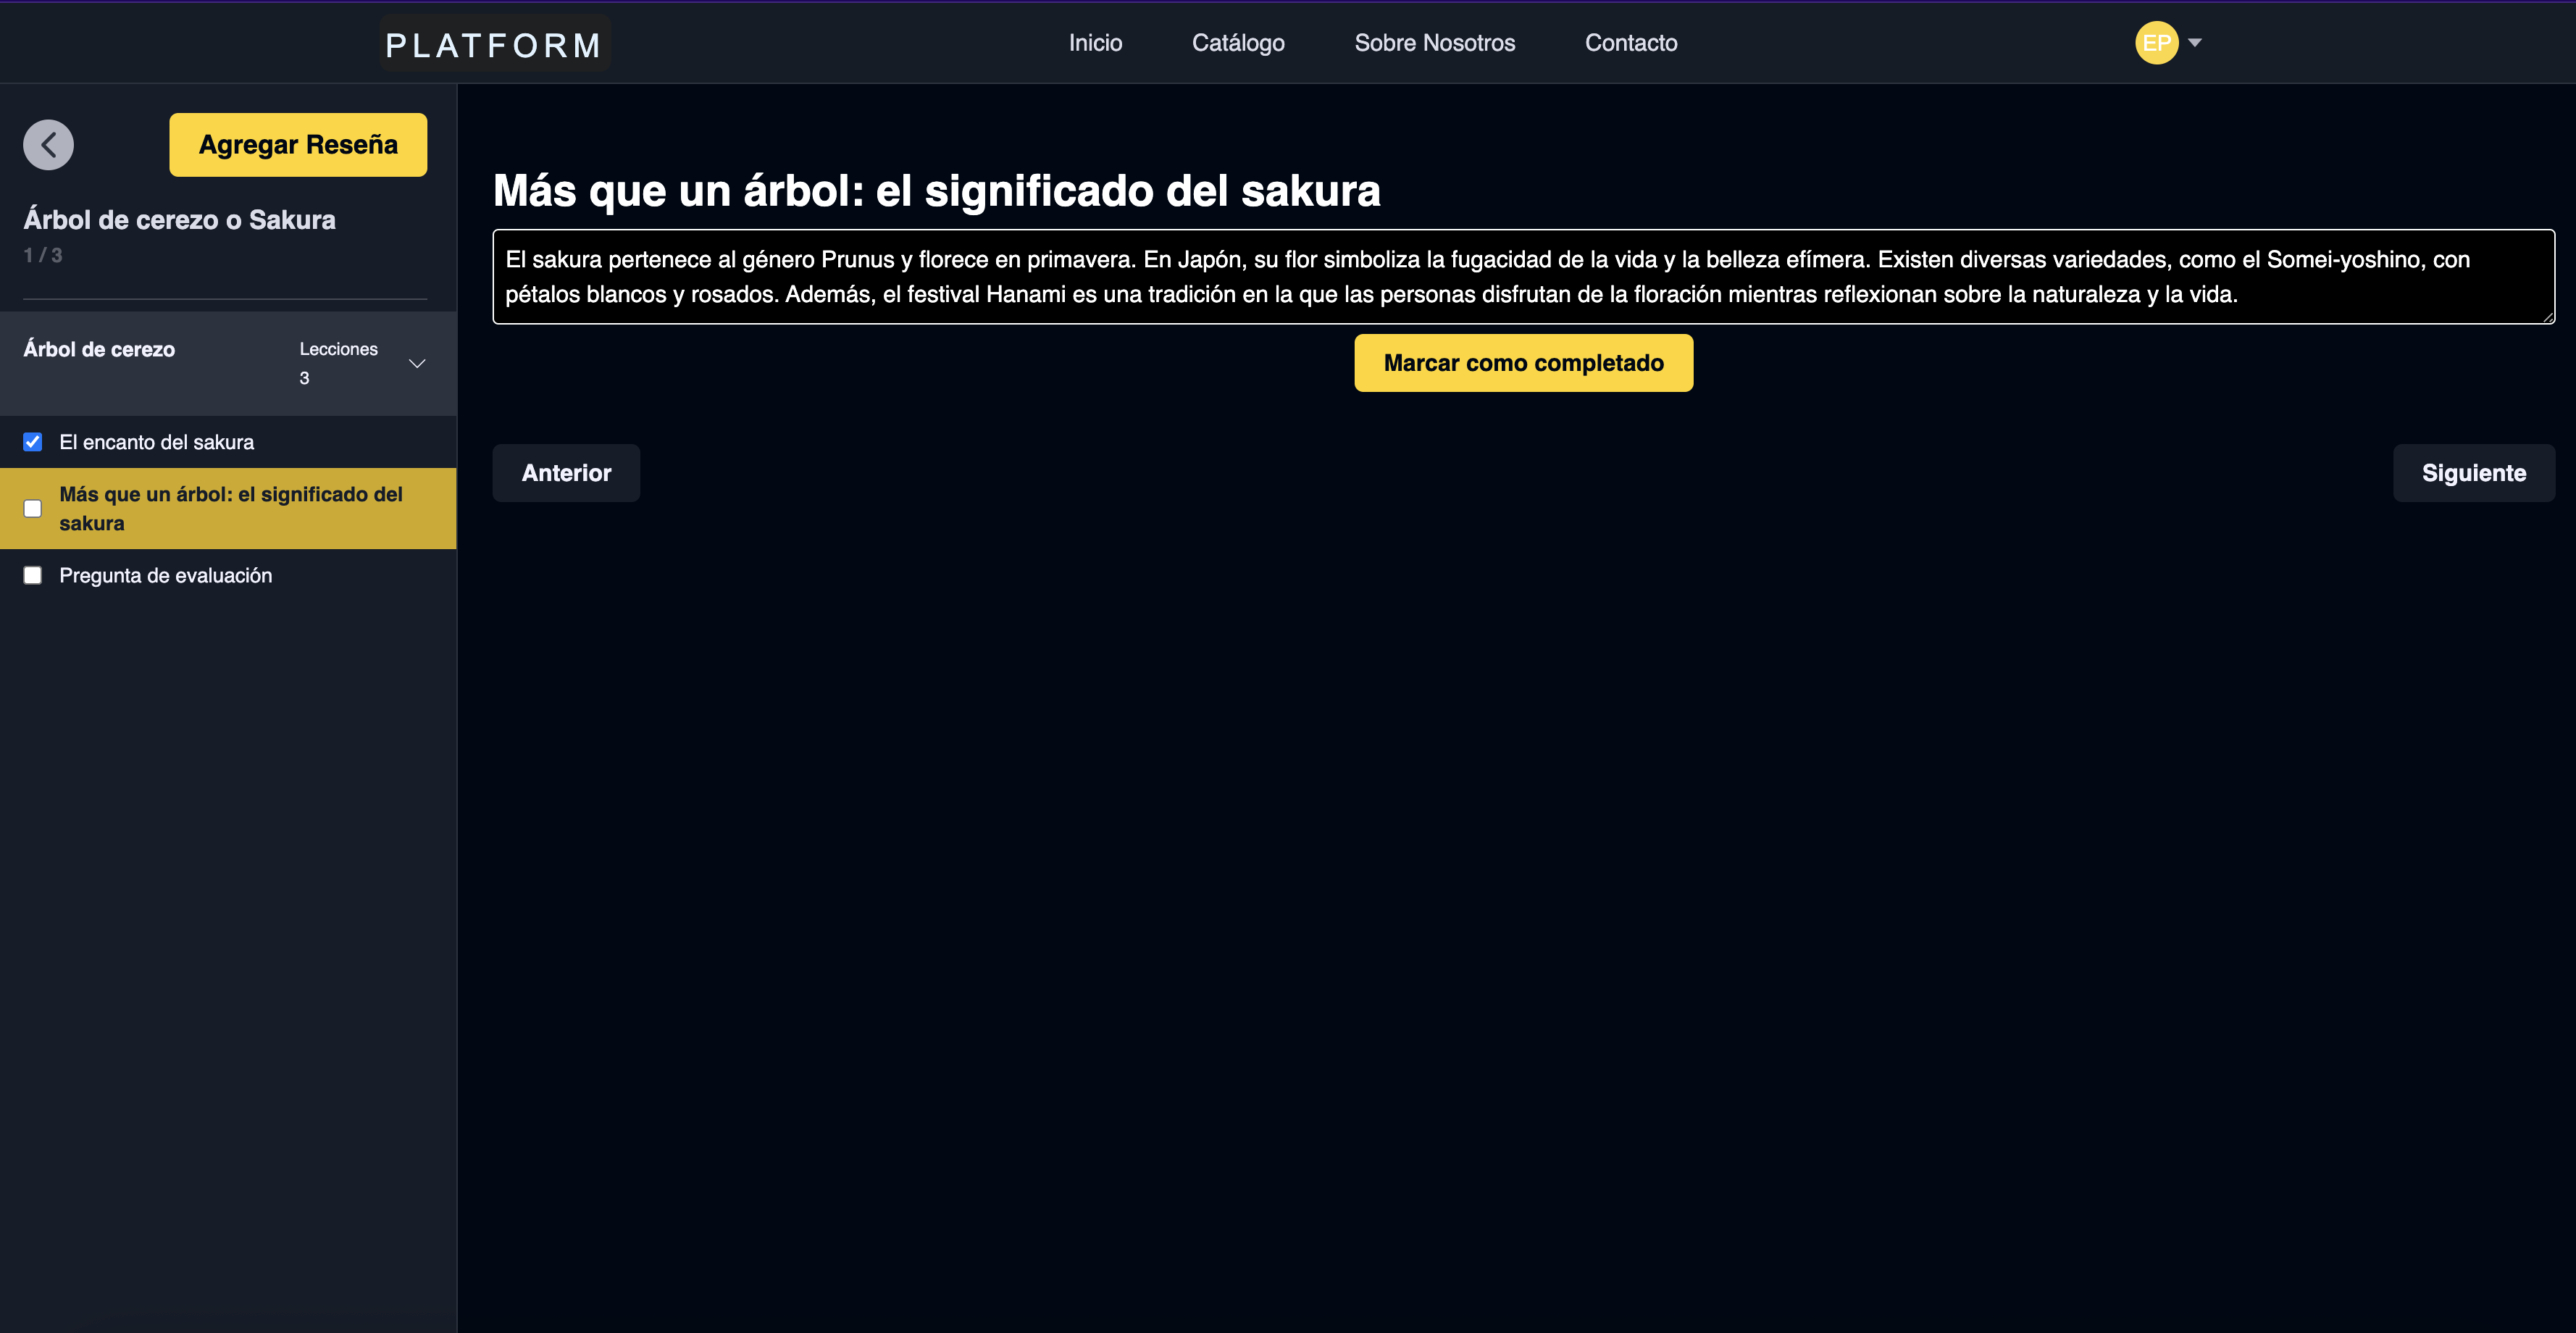
\includegraphics[width=\linewidth]{leccion/leccion_02.png}
    \caption{Lección tipo texto}
    \label{fig:leccion_texto}
\end{figure}

\begin{figure}[H]
    \centering
    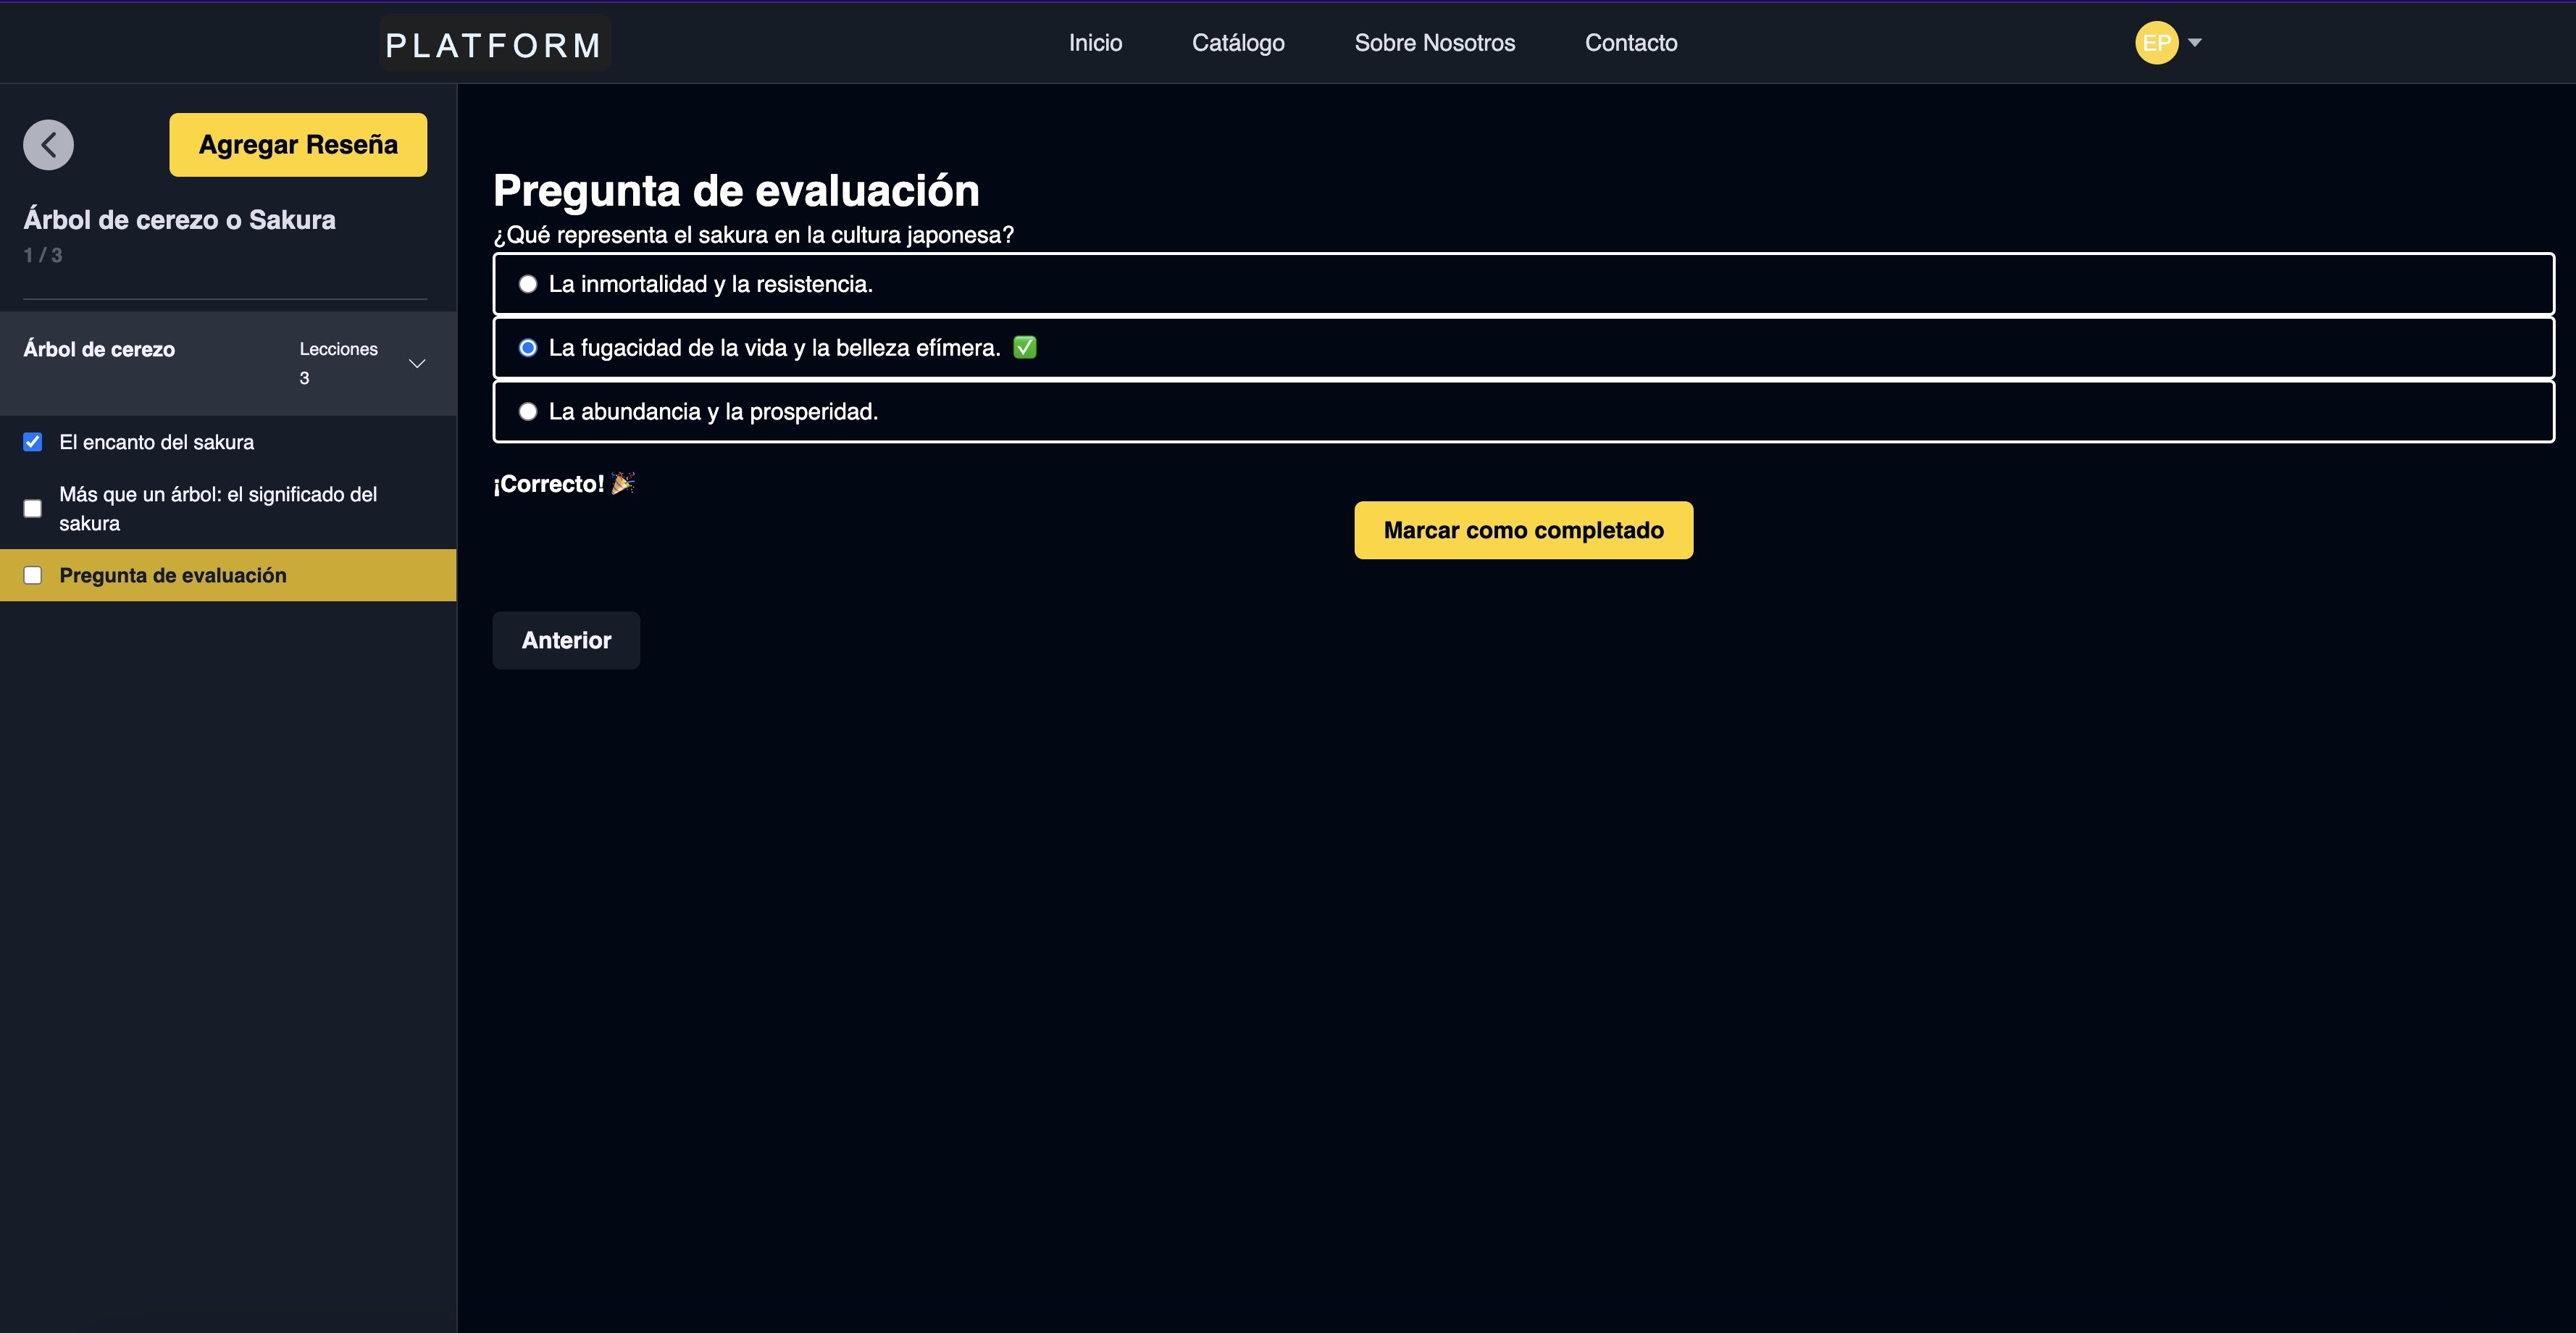
\includegraphics[width=\linewidth]{leccion/leccion_03.png}
    \caption{Lección tipo opción mútiple}
    \label{fig:leccion_opcion_multiple}
\end{figure}

\section{Integración con Telegram en Imágenes}

\begin{figure}[H]
    \centering
    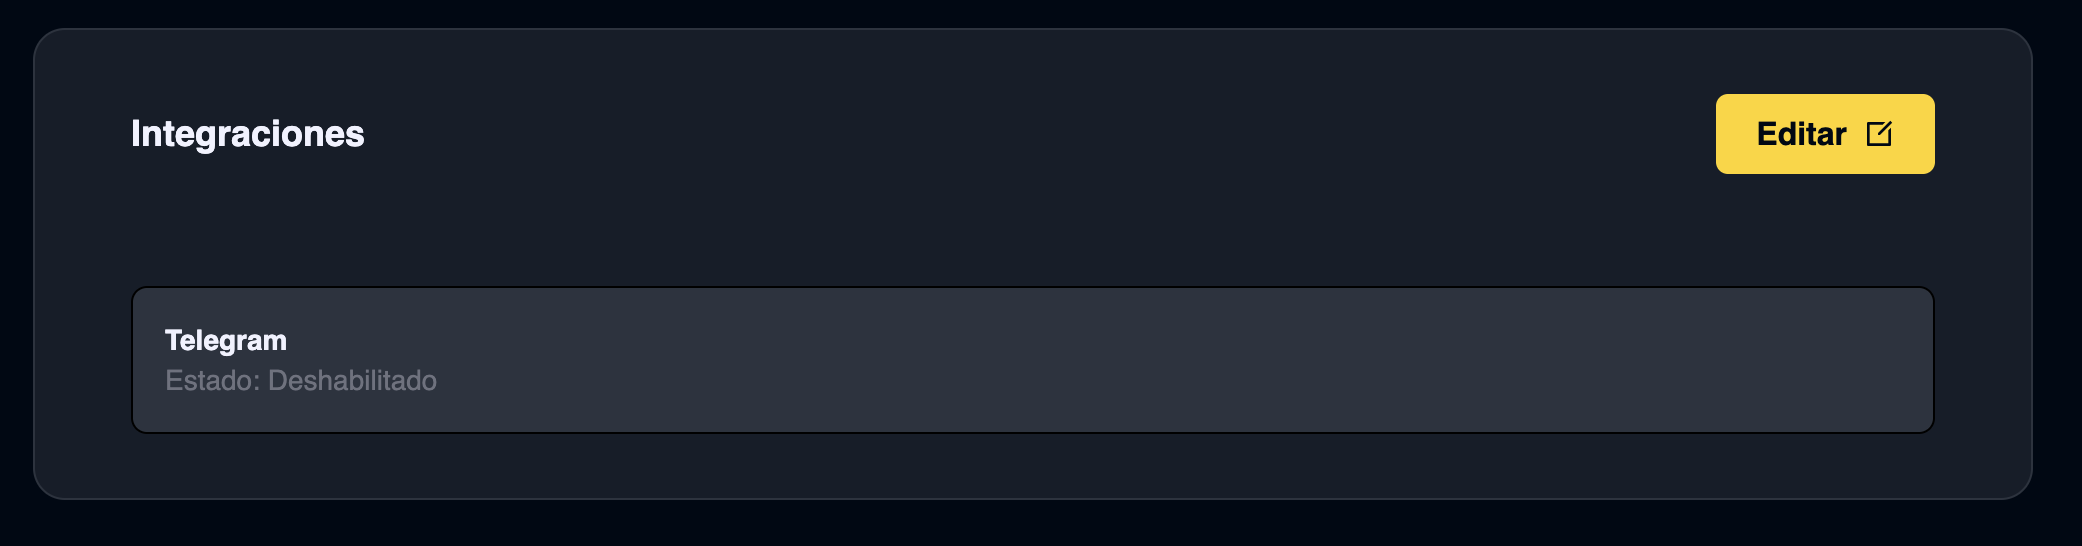
\includegraphics[width=\linewidth]{integracion_telegram/integracion_telegram_01.png}
    \caption{Integración deshabilitada}
    \label{fig:integracion_telegram_deshabilitada}
\end{figure}

\begin{figure}[H]
    \centering
    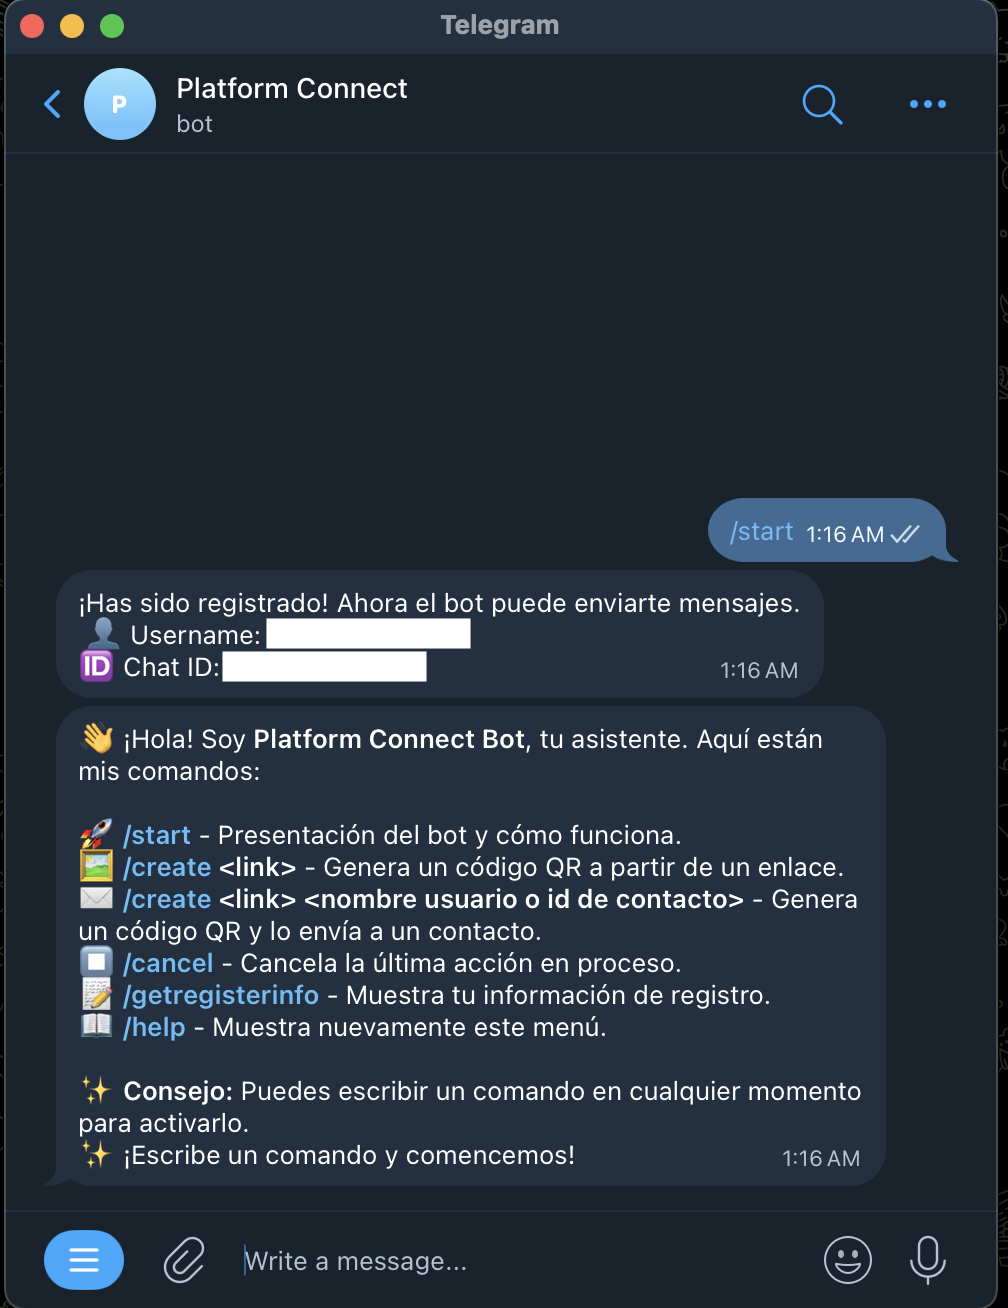
\includegraphics[width=\linewidth]{integracion_telegram/integracion_telegram_03.png}
    \caption{Registro de usuario en el bot}
    \label{fig:integracion_telegram_registro_bot}
\end{figure}

\begin{figure}[H]
    \centering
    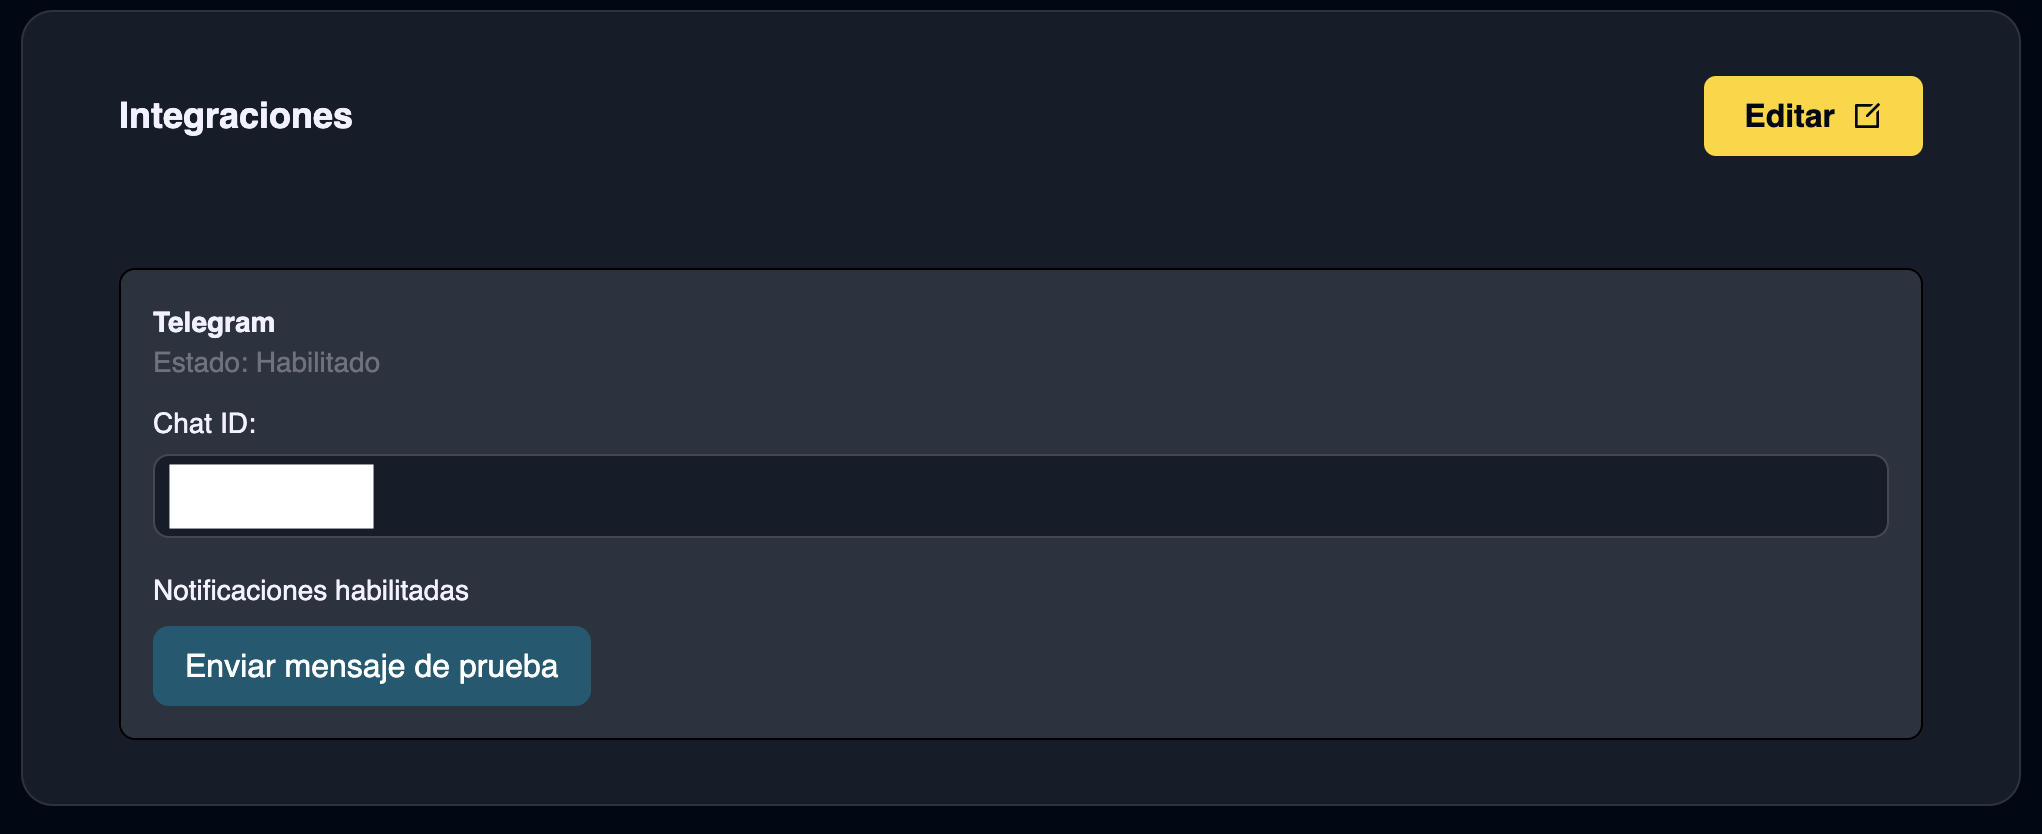
\includegraphics[width=\linewidth]{integracion_telegram/integracion_telegram_04.png}
    \caption{Integración habilitada}
    \label{fig:integracion_telegram_habilitada}
\end{figure}

\section{Integración con Sistema de Correos Electrónicos en Imágenes}

\begin{figure}[H]
    \centering
    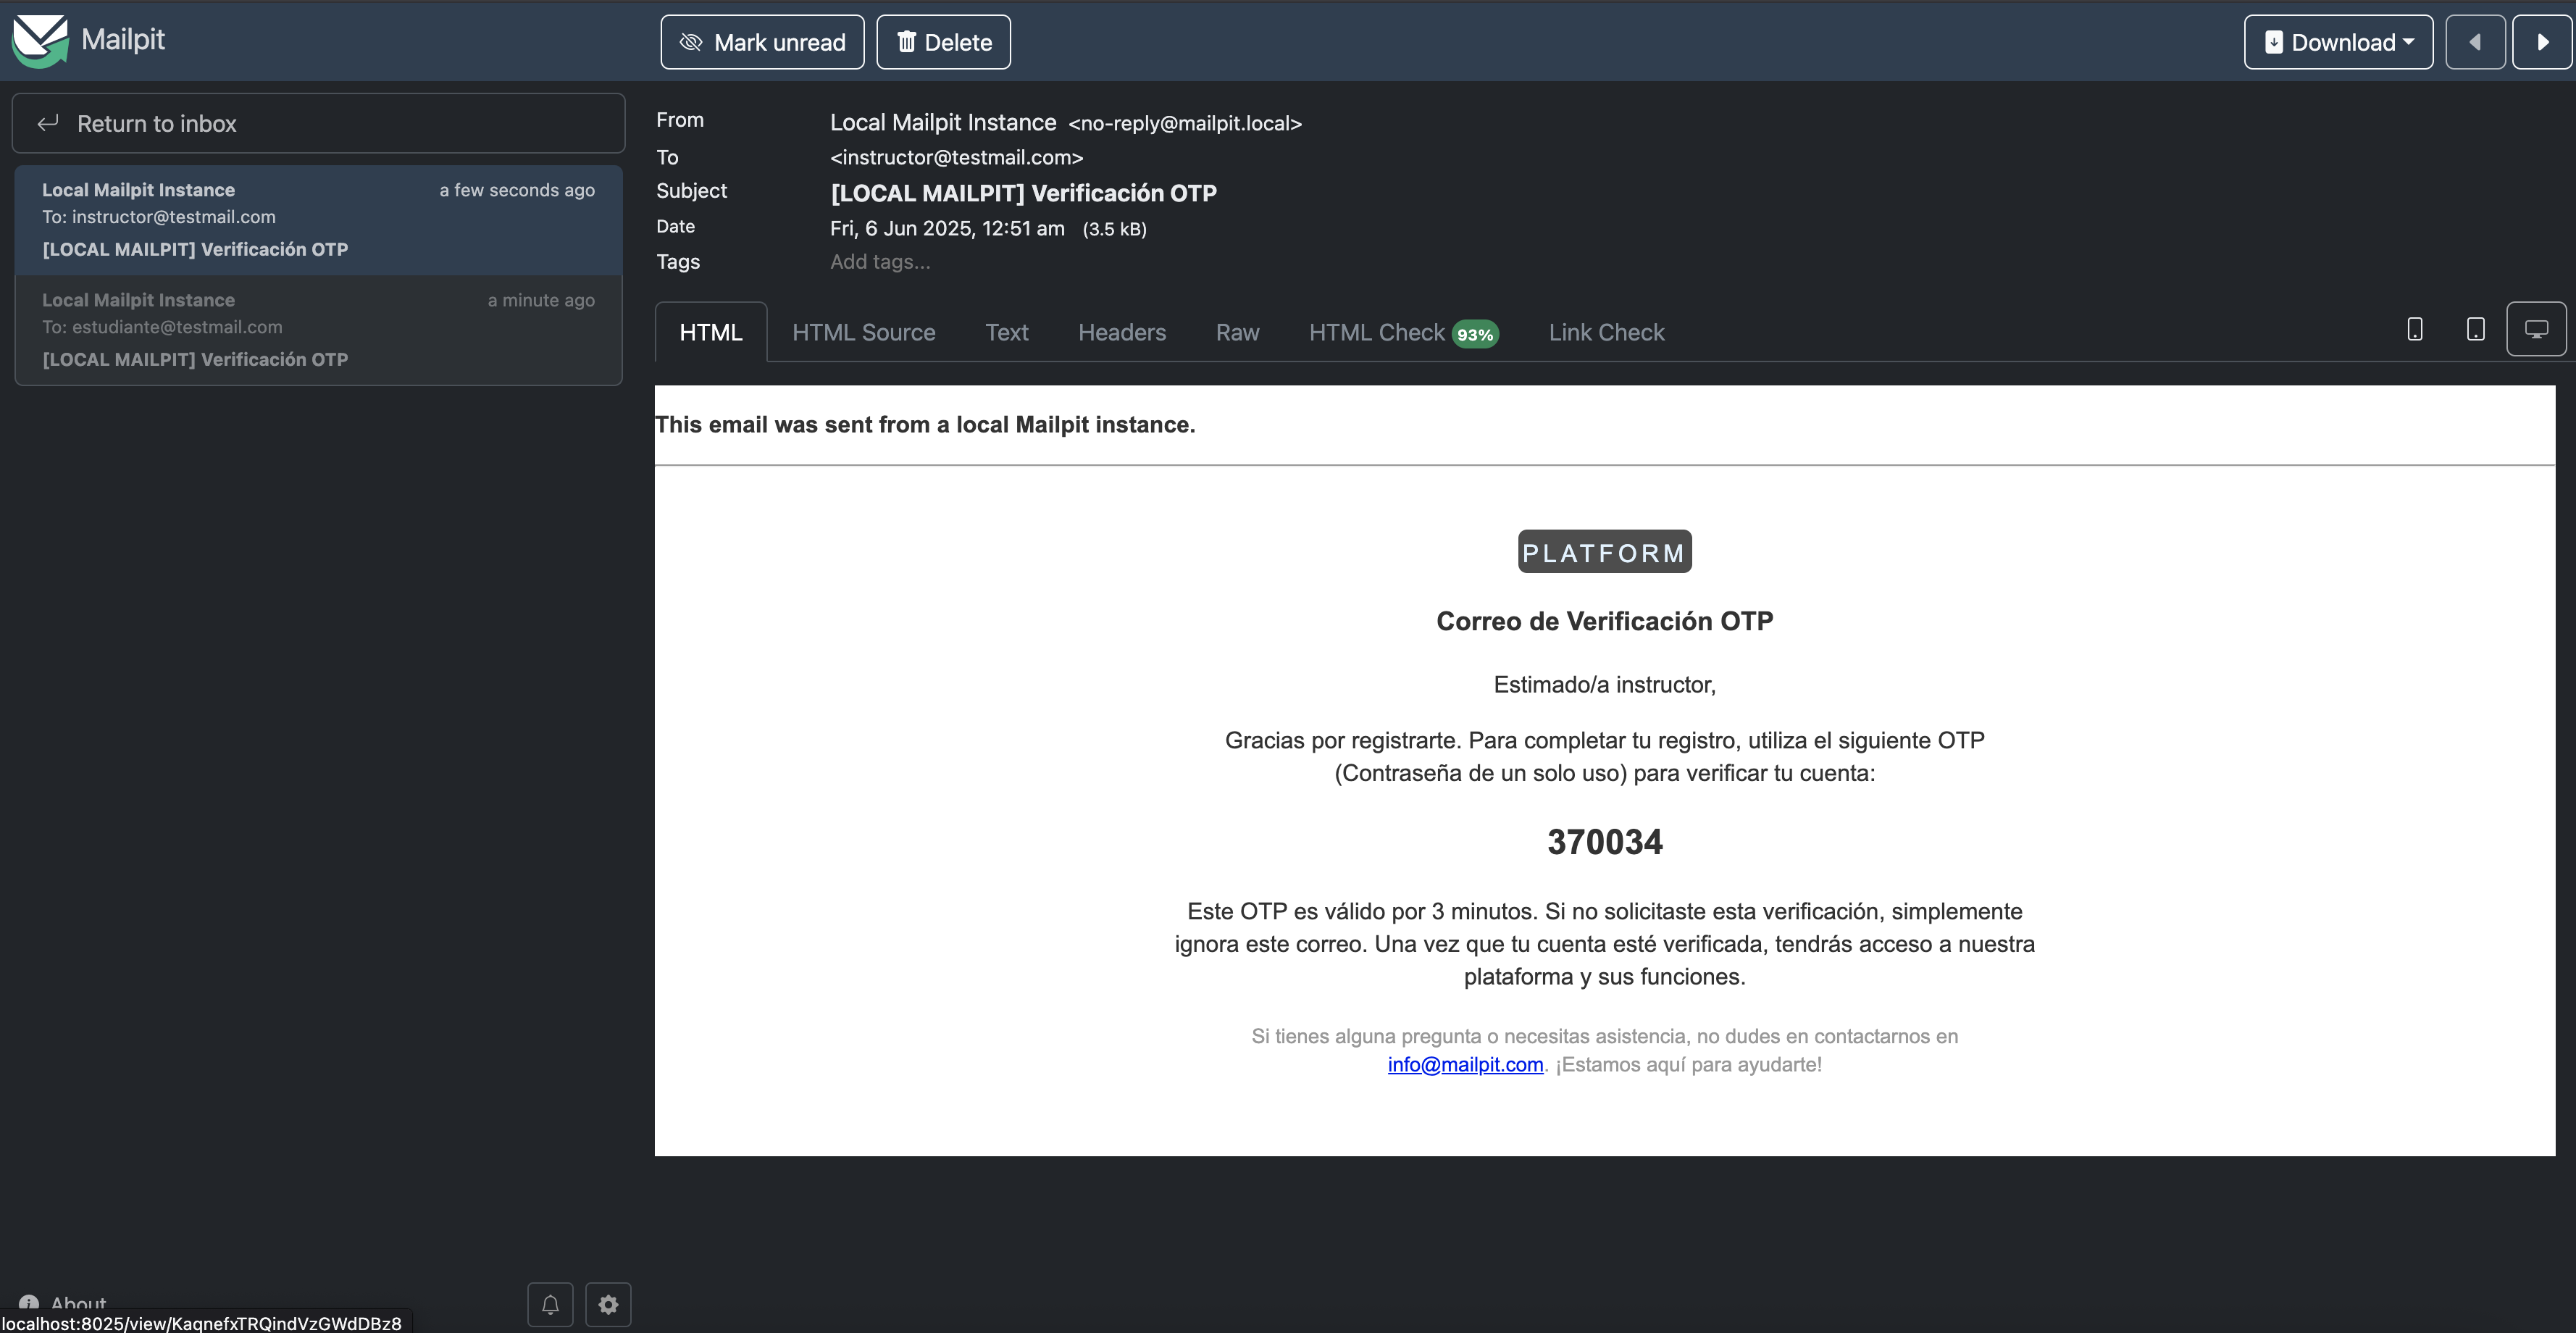
\includegraphics[width=\linewidth]{mail/mail_01.png}
    \caption{Correo de OTP}
    \label{fig:correo_electronico_otp}
\end{figure}
\begin{figure}[H]
    \centering
    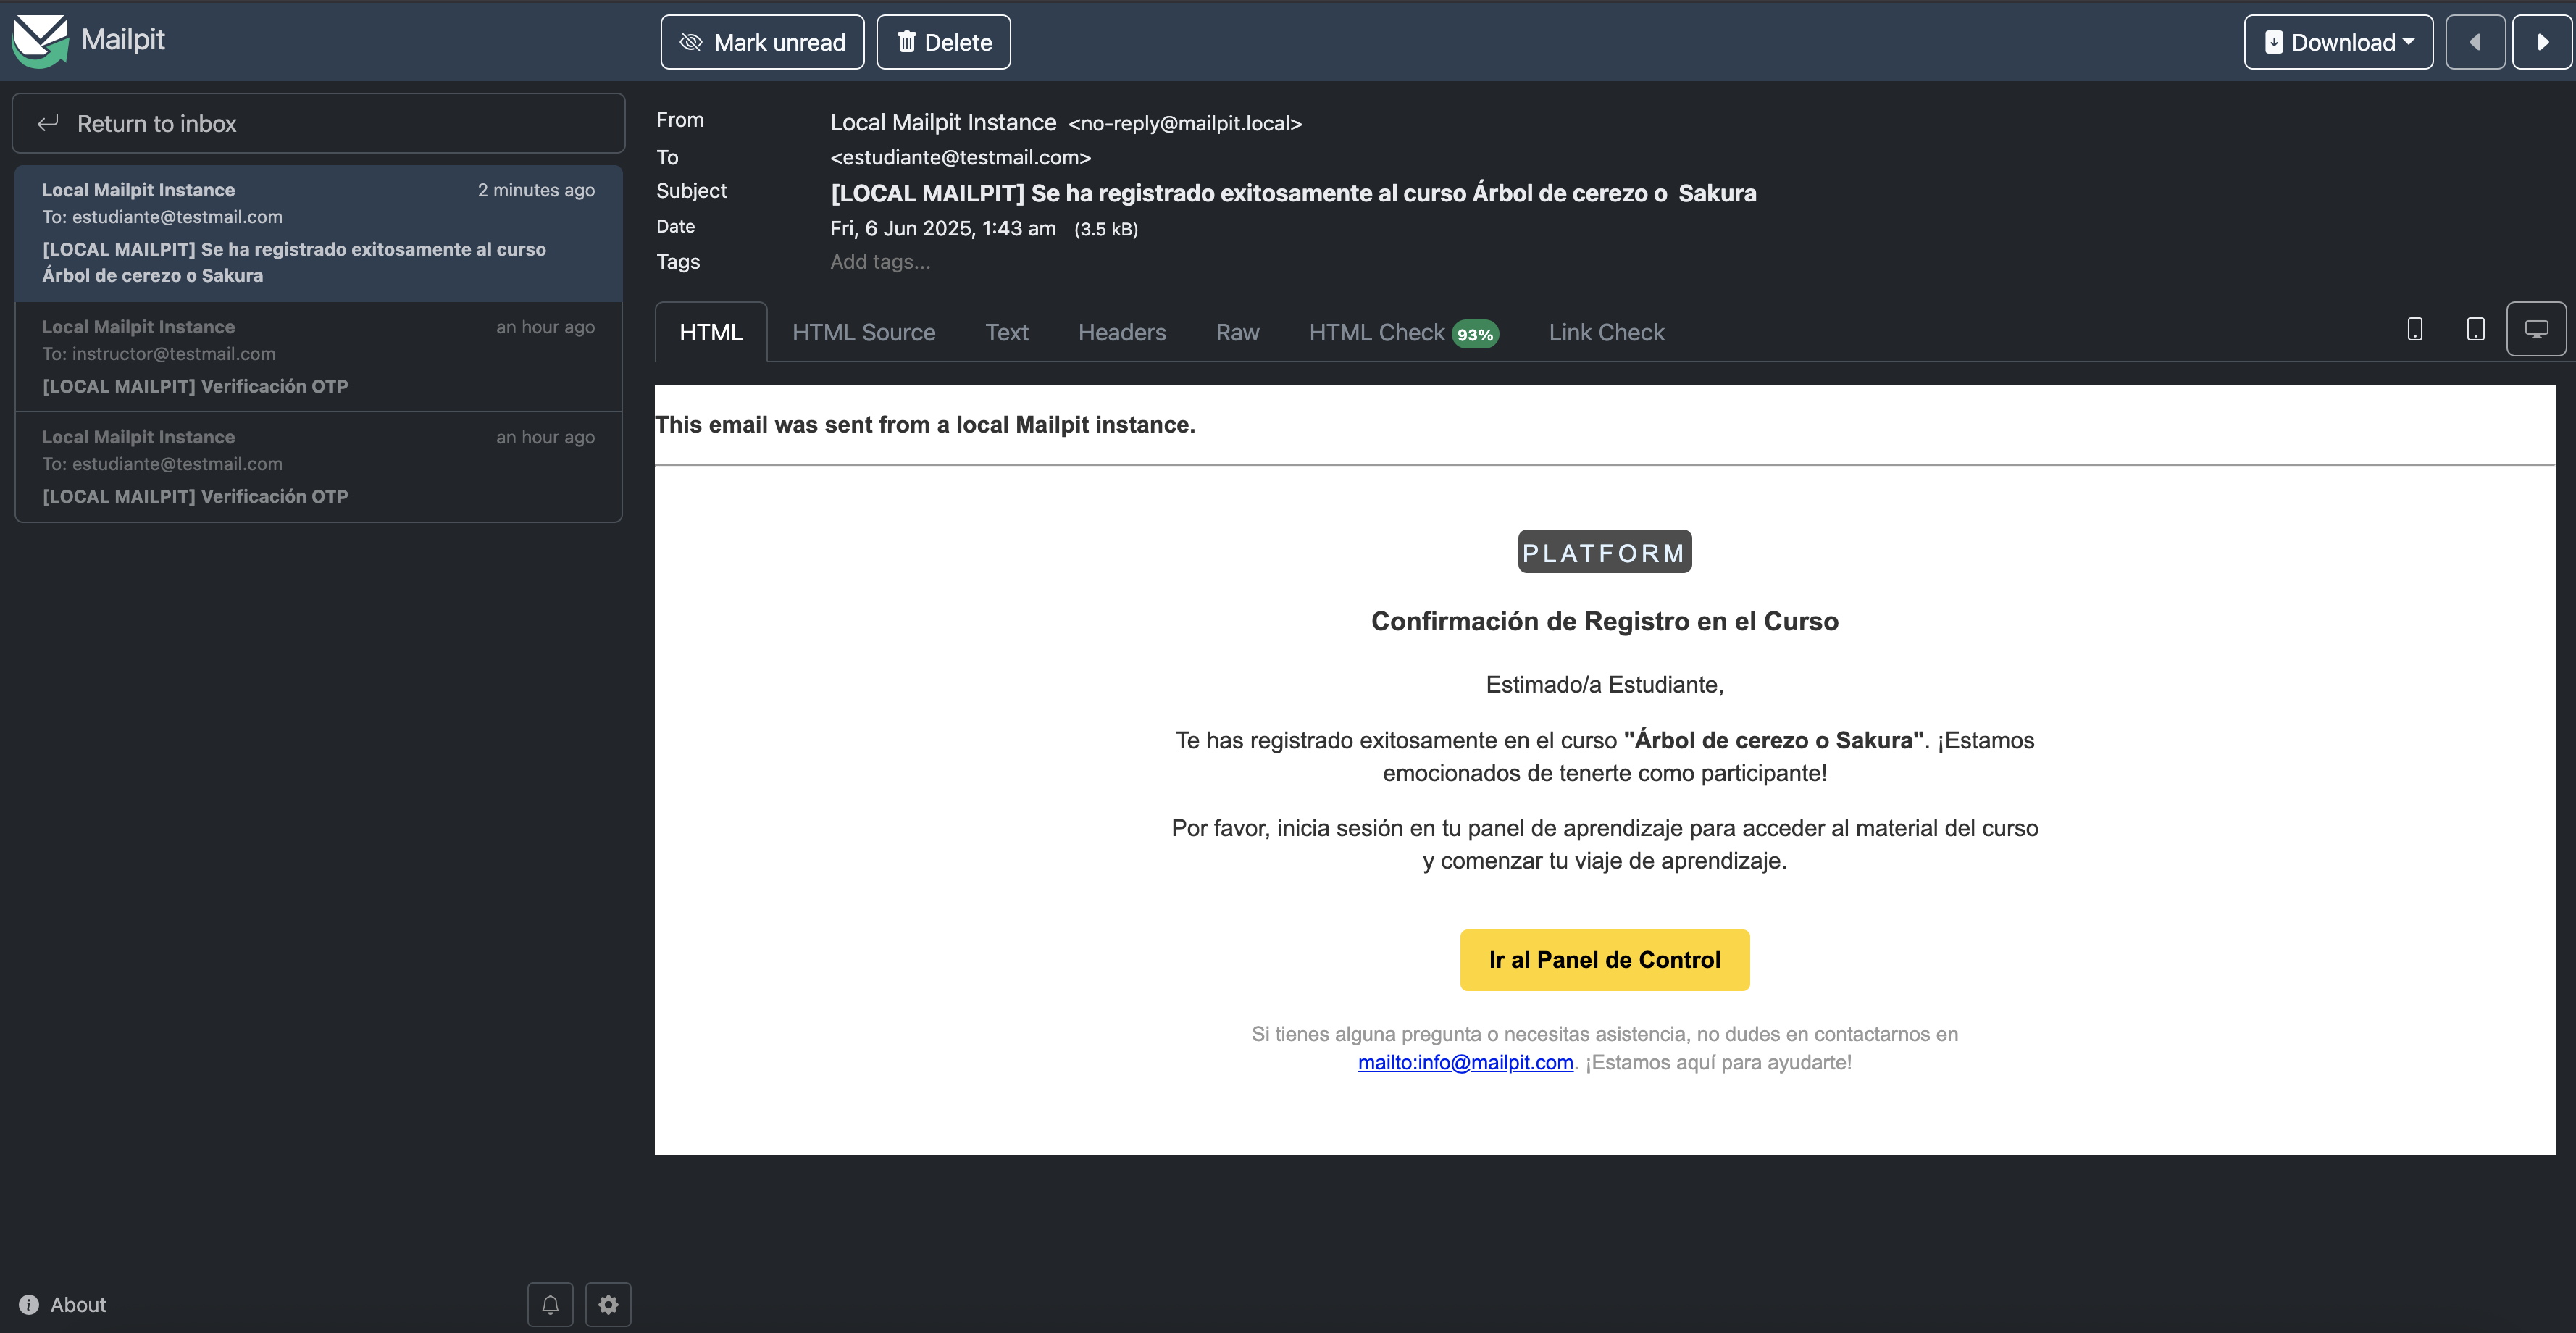
\includegraphics[width=\linewidth]{mail/mail_02.png}
    \caption{Correo de confirmación de registro a curso}
    \label{fig:correo_electronico_confirmacion_registro_curso}
\end{figure}


\section*{Reconocimientos}
\blindtext
\begin{comment}
Deseo expresar mi más profundo agradecimiento a mis padres, cuyo apoyo incondicional y acompañamiento han sido
fundamentales a lo largo de toda mi carrera.

Asimismo, extiendo mi gratitud a la Universidad de Palermo (UP), a sus docentes y autoridades, por proporcionarme
las herramientas necesarias para la realización de este trabajo, contribuyendo significativamente a mi formación académica.

Quiero hacer una mención especial al Magíster Javier Rabuch, Director de las carreras de Inteligencia Artificial,
por su valiosa orientación y apoyo durante el desarrollo de esta investigación, tanto en su rol de profesor como
en su función de tutor. Su guía ha sido clave en el proceso de este estudio.
\end{comment}

\begin{comment}
	\begin{thebibliography}{5}
		\bibitem{IEEEhowto:kopka}
		H.~Kopka and P.~W. Daly, \emph{A Guide to \LaTeX}, 3rd~ed.\hskip 1em plus
		0.5em minus 0.4em\relax Harlow, England: Addison-Wesley, 1999.
	\end{thebibliography}
\end{comment}

\bibliographystyle{IEEEtran}
\bibliography{bib/IEEEabrv,bib/references}
% if no citation then you have to use the following command to show references:
\nocite{*}

\begin{IEEEbiography}[
        {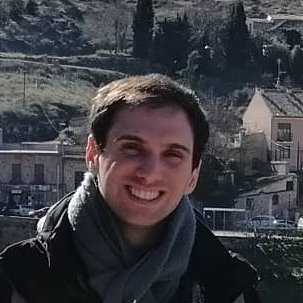
\includegraphics[width=1in,height=1.25in,clip,keepaspectratio]{images/author.jpg}}
    ]
    {Andrés Isaac Biso} es estudiante de la carrera de Licenciatura en Informática en la Universidad de Palermo (UP).
    Posee el título de Analista Universitario en Sistemas otorgado por la misma institución.
    Con casi diez años de experiencia como desarrollador de software, ha trabajado con clientes nacionales e internacionales,
    desarrollando soluciones tecnológicas adaptadas a diversas necesidades empresariales.
\end{IEEEbiography}


\end{document}
